
\chapter{State of the Art}

The basic ideas of cloud-native architecture and best practices for achieving a secure, scalable and distributed architecture for AI models are explained in detail in this chapter. A solid understanding of these underlying concepts is required to fully comprehend the approaches identified and explored in the literature review.

\section{Cloud-Native Architectures}

Cloud-native technologies have transformed the landscape of application development, deployment and management by leveraging cloud environments to their fullest potential \cite{r9}. These technologies focus on creating applications as a collection independently deployable services which are loosely coupled, allowing the integration of modules within a cloud-native infrastructure \cite{r10}. Key principles of this approach include containerization, microservices architecture, declarative APIs, continuous integration and delivery \abk{CI/CD}{Continuous Integration and Delivery} and infrastructure as code \abk{IAS}{Infrastructure as Code} \cite{r11}. By embracing cloud-native methodologies, organizations can achieve greater scalability, agility and resilience, enabling the delivery of innovative and dependable software solutions \cite{r12}. In modern software development, scalability and resilience are paramount due to the heightened demand for applications that are both highly available and responsive \cite{r13}. Scalability is the capability of a system to manage varying workloads effectively, accommodating sudden traffic spikes or a steady increase in users \cite{r14}. Resilience ensures that applications continue to function despite failures or disruptions in the underlying infrastructure \cite{r15}. To meet user expectations and ensure business continuity while competing in digital economy, scalability and resilience qualities must be achieved.



\section{Scope and Relevance}

Although this thesis report deals with the principles of secure, scalable and distributed computing, in particular the topic of authentication and authorization using the principles of RBAC and SSO. It also looks at the Ray framework for scalability in distributed computing. Ray is particularly effective in this area because, in addition to the ease of use of the \abk{API}{Application Programming Interface}, it provides easy scalability, effective and resilient fault tolerance and high performance. All of these features make Ray a worthy tool for developers and organizations that want to build highly efficient and reliable distributed applications. Thus, when considering the questions of secure and scalable distributed computation, it is paramount to achieve proper authentication and authorization. Computer security is in a state of flux constantly, with examples of effective solutions include RBAC as well as SSO, both of which help in the protection of resources as well as ease the management of user details. RBAC in Kubernetes, involves the use of RoleBinding and ClusterRoleBinding resources to enable efficient management of access control by namespace and cluster \cite{burns2022Kubernetes}. SSO improves the user experience and security since the user only has to provide the credentials once and the system provides access rights to multiple applications and services which helps to streamline the access control and ensure that the administrative overhead is also reduced \cite{jangda2020sso}. Through embedding the identified Ray framework in combination with such sound RBAC and SSO solutions, it is possible to provide organizations with the secure, large-scale and efficient distributed computation environments. \cite{zaharia2012resilient, moritz}


\section{Fundamentals of Cloud-Native Architecture}

Cloud-native technologies consist a set of methodologies, practices and tools designed for cloud environments. These include containerization and microservice architectures, which allows to achieve scalability, agility and resilience in cloud platforms to deliver cutting-edge and well grounded software solutions. \cite{r16}

\subsection{Containerization}

Containerization is a technique that packages an application with all its necessary dependencies into a lightweight, single unit called container. This approach guarantees consistent performance across different computing environments by encapsulating all components required to execute the application, such as libraries, dependencies and configuration files within the container. Unlike virtual machines, containers share the host system kernel, making them more efficient in terms of resource utilization and startup time. Docker is one of the most widely used containerisation platforms, providing tools for creating, managing and deploying containers, enabling developers to build, test and deploy applications with ease and consistency. The containers architecture, including their interaction with the host system, can be visualized in \autoref{fig:Container Architecture}. \cite{Docker_container}

\captionsetup{justification=centering}
\begin{figure}[h]
\centering
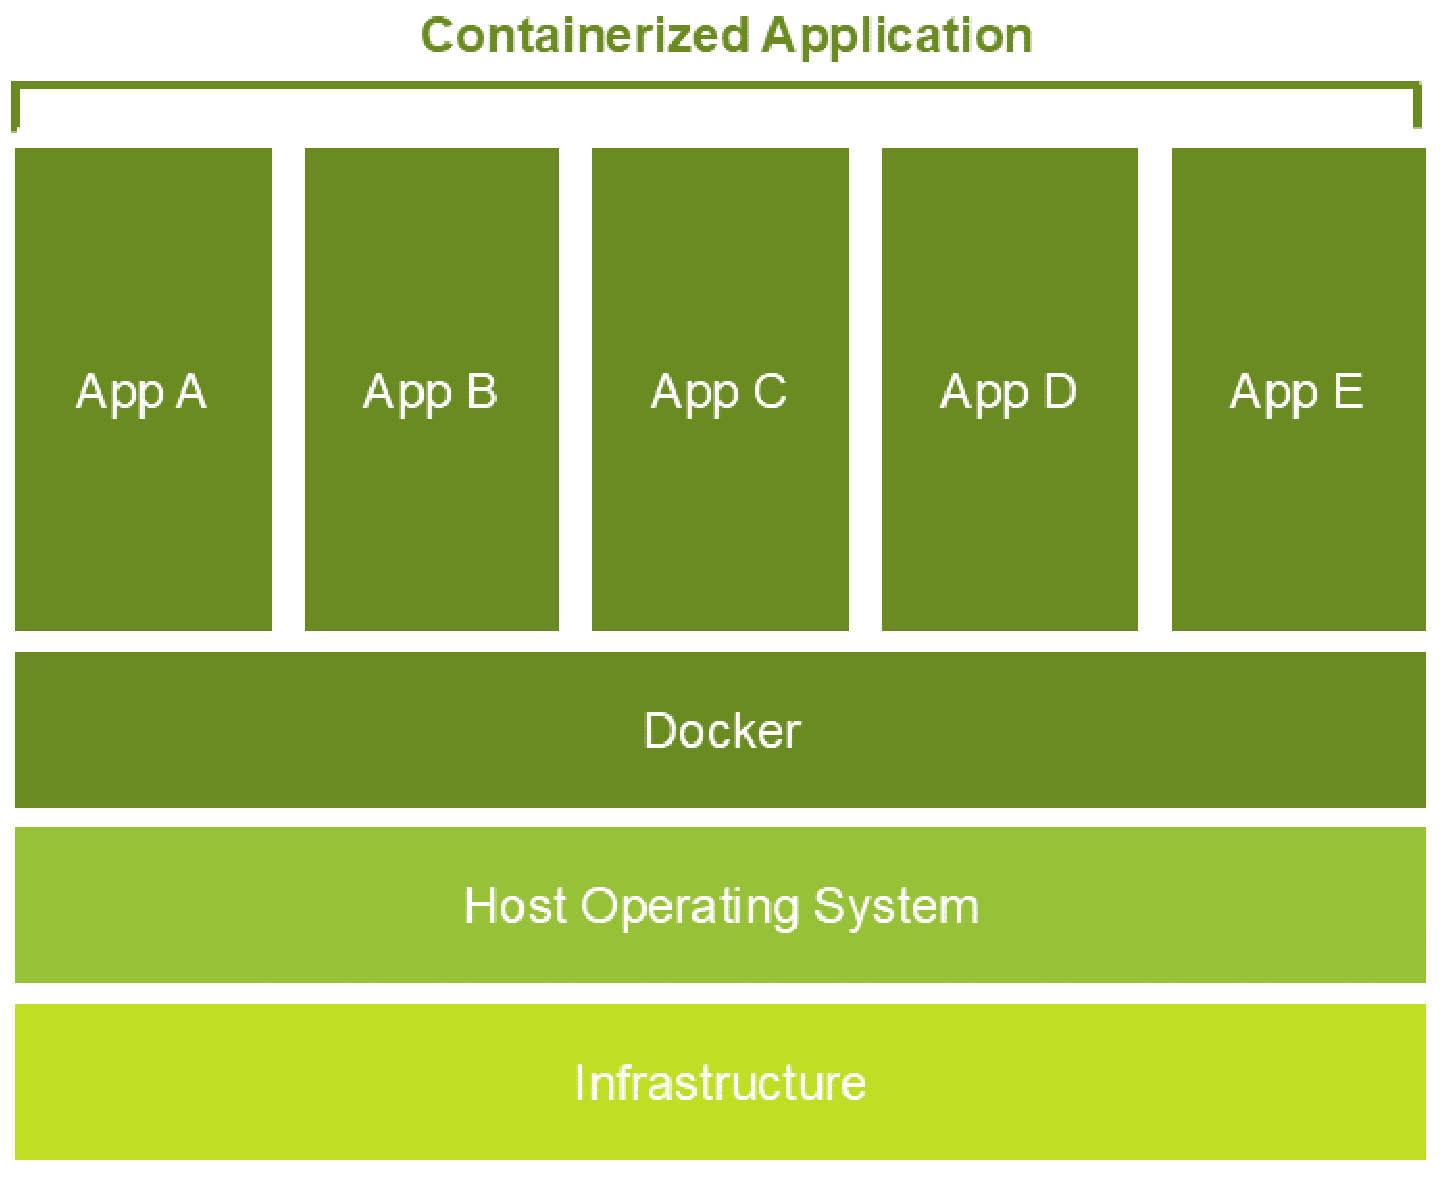
\includegraphics[width=0.8 \linewidth]{Thesis/Figures/Slide3.pdf}
\caption{\label{fig:Container Architecture}Container Architecture \cite{Docker_container}}
\end{figure}

\vspace{0.2cm}

The architecture of containers allows for significant improvements in development workflows and operational efficiency \cite{Kubernetes_doc}. By isolating applications and their dependencies from the host system, containers eliminate the common problem of \texttt{dependency hell} and environment inconsistencies \cite{Kubernetes_doc}. This isolation also enhances security by limiting the applications access to the host system \cite{Kubernetes_doc}. Additionally, container orchestration tools like Kubernetes have emerged to manage the deployment, scaling and operation of containerized applications across clusters of machines, further enhancing the robustness and scalability of containerized solutions \cite{Kubernetes_doc}. Overall, containerization has revolutionized the way applications are developed, deployed and managed, making it a cornerstone technology in modern DevOps practices \cite{redhat_docs}.

\textbf{Docker}

Docker is an open source platform that simplifies the development, deployment and distribution of applications. It packages applications and their necessary dependencies into standardised units called containers. These containers run in isolation on top of the operating system kernel, providing a lightweight and efficient environment for running code. Docker enables developers to easily create, manage and deploy containers, allowing applications to run anywhere without modification and ensuring seamless portability across environments. In addition, Docker integrates with third party tools to improve the deployment and management of containers, particularly in cloud-native environments. Docker works on a client server model, where the Docker client sends requests to the Docker server, which handles those requests. The platform consists of several key components including the Docker client, Docker server, Docker images, Docker registries and Docker containers. Docker images are created using read-only templates, with a base image such as Ubuntu serving as the foundation. Images can either be created from scratch or modified. Docker files provide an automated method of building images by following a set of instructions. These images are stored in Docker registries, such as Docker Hub, which can be public or private. Finally, Docker containers are created from Docker images and encapsulate everything needed to run an application in an isolated environment. This isolation ensures consistency and reliability across different platforms, making Docker a powerful tool for modern software development. \cite{rad2017introduction}

\subsection{Microservices Architecture}

Microservices architecture is an approach where applications are divided into small, independently deployable services, each responsible for handling different business functions, as shown in \autoref{fig:Microservice Architecture}. These services interact with each other using well-defined APIs and communication protocols, allowing developers to focus on individual components separately. This approach promotes scalability, flexibility and modularity by allowing teams to develop and scale services independently, resulting in faster development cycles and improved fault isolation. \cite{r22}

\clearpage

\captionsetup{justification=centering}
\begin{figure}[h]
\centering
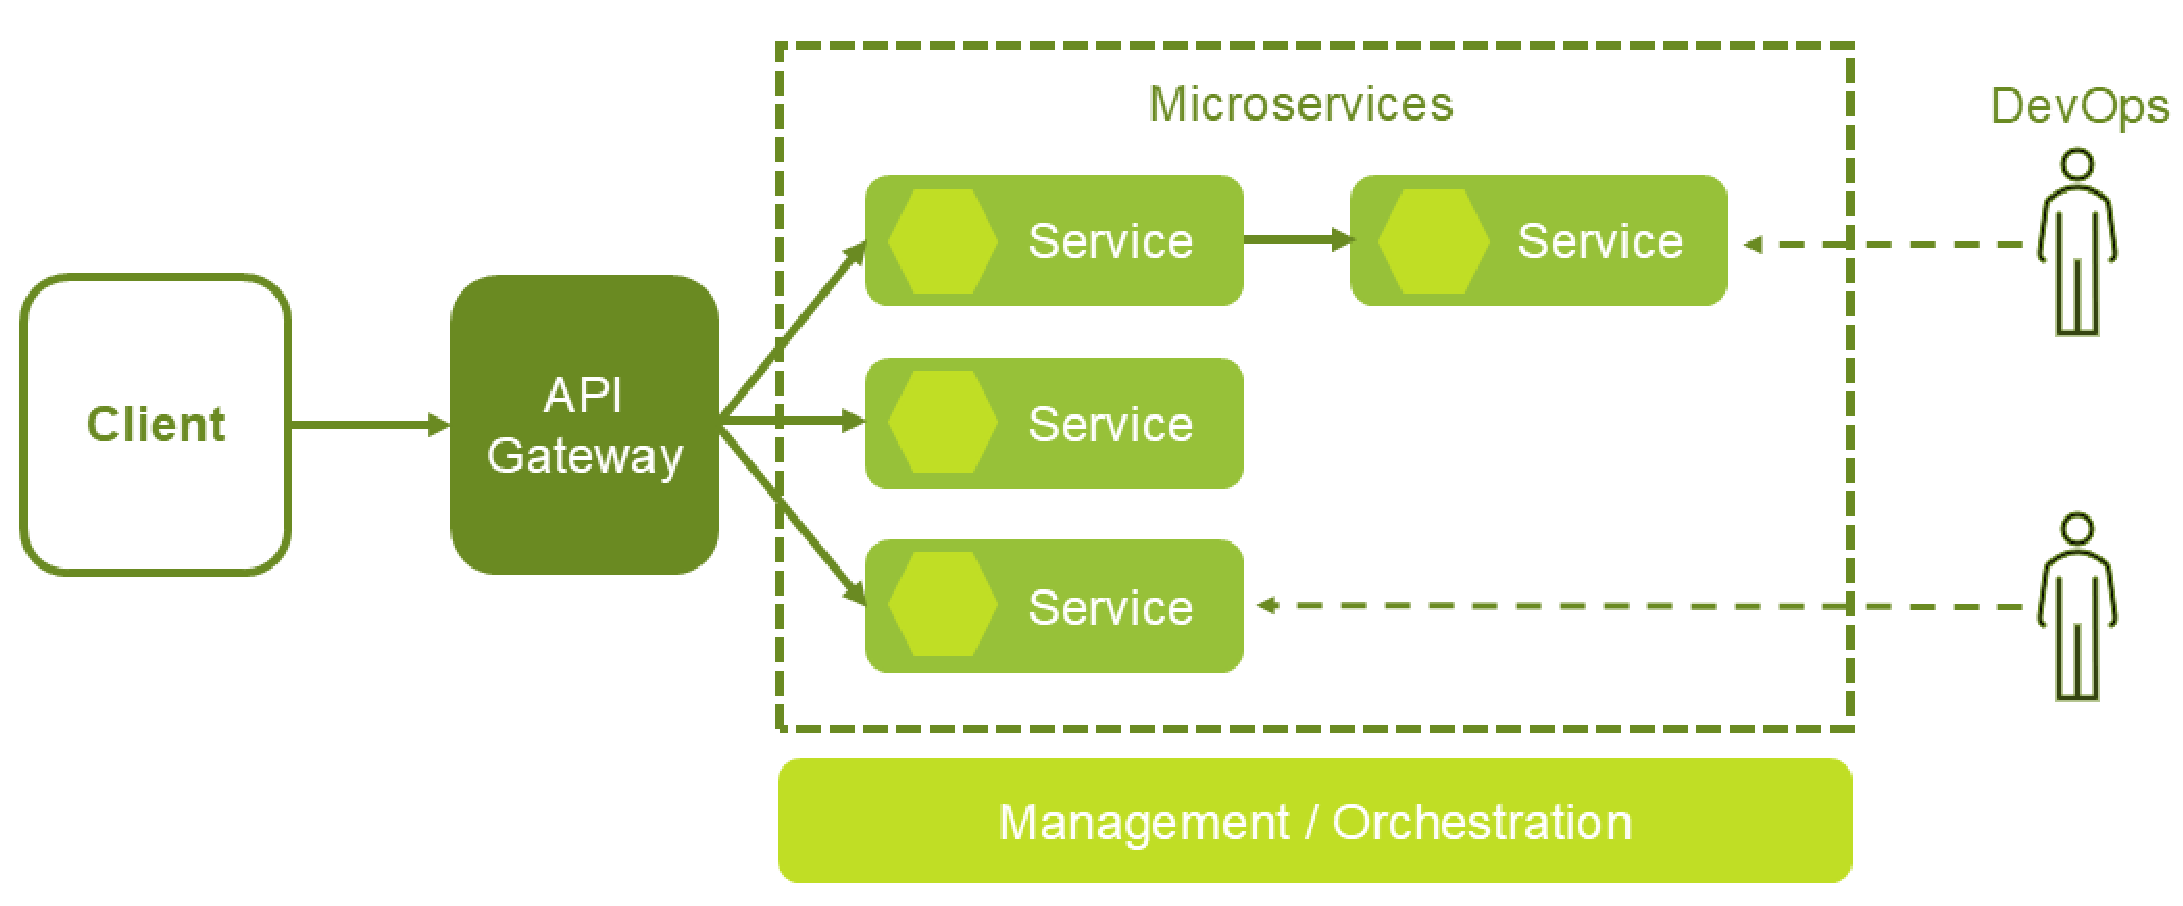
\includegraphics[width=0.9 \linewidth]{Thesis/Figures/Slide4.pdf}
\caption{\label{fig:Microservice Architecture}Microservice Architecture \cite{r23}}
\end{figure}


\subsection{Container Orchestration}

Container orchestration remains essential for scalable and automated coordination of microservice architectures, managing the lifecycle of containers and services in a compute cluster. Typically, end users submit their jobs to a cluster manager, one of the core components of the orchestration system. The cluster manager is responsible for assigning tasks to worker nodes within the cluster. These clusters, composed of either physical or virtual machines, execute the required tasks. An application or job often relies on multiple services, each running in containers with diverse tasks. Container orchestrators provide an abstraction layer that simplifies the management of complex environments and architectural solutions, whether for client facing infrastructures or cloud services. Popular on premise orchestrators include Kubernetes, Borg and Mesos, typically installed and configured as standalone software. In the cloud, Google Kubernetes engine \abk{GKE}{Google Kubernetes Engine}, Microsoft Azure Kubernetes service \abk{AKS}{Azure Kubernetes Service} and Amazon elastic Kubernetes service \abk{EKS}{Elastic Kubernetes Service} are widely used hosted solutions with predefined, easily configurable setups. \cite{carrion2022Kubernetes}

Another core component of the container orchestrators is the scheduling module, which embodies the component in question and aimed towards finding which node should execute an incoming task considering various factors which include availability of resources, necessary node affinities, or location of the data to be processed. Furthermore, there is also the rescheduler component that assists in transforming tasks location to group loads or optimise the usage of resource. Others consist of the resource allotment module through which resources of the cluster are assigned either dynamically or even statically and the load distribution module which enforces the distribution of the submitted tasks in line with some specified criteria within the cluster. The autoscaling module where resources are adjusted either horizontally or vertically based on the workload within the cluster. Also, the admission control module tries to guarantee that the resources requested fit within the cluster’s capacity, whereas the accounting and monitoring modules provide information regarding resource utilization and node health, respectively, for system dependability and fault tolerance purposes as shown in \autoref{fig:Container Orchestration}. These components in total deliver a strong environment for optimal and distributed container processes. \cite{carrion2022Kubernetes}


\captionsetup{justification=centering}
\begin{figure}[h]
\centering
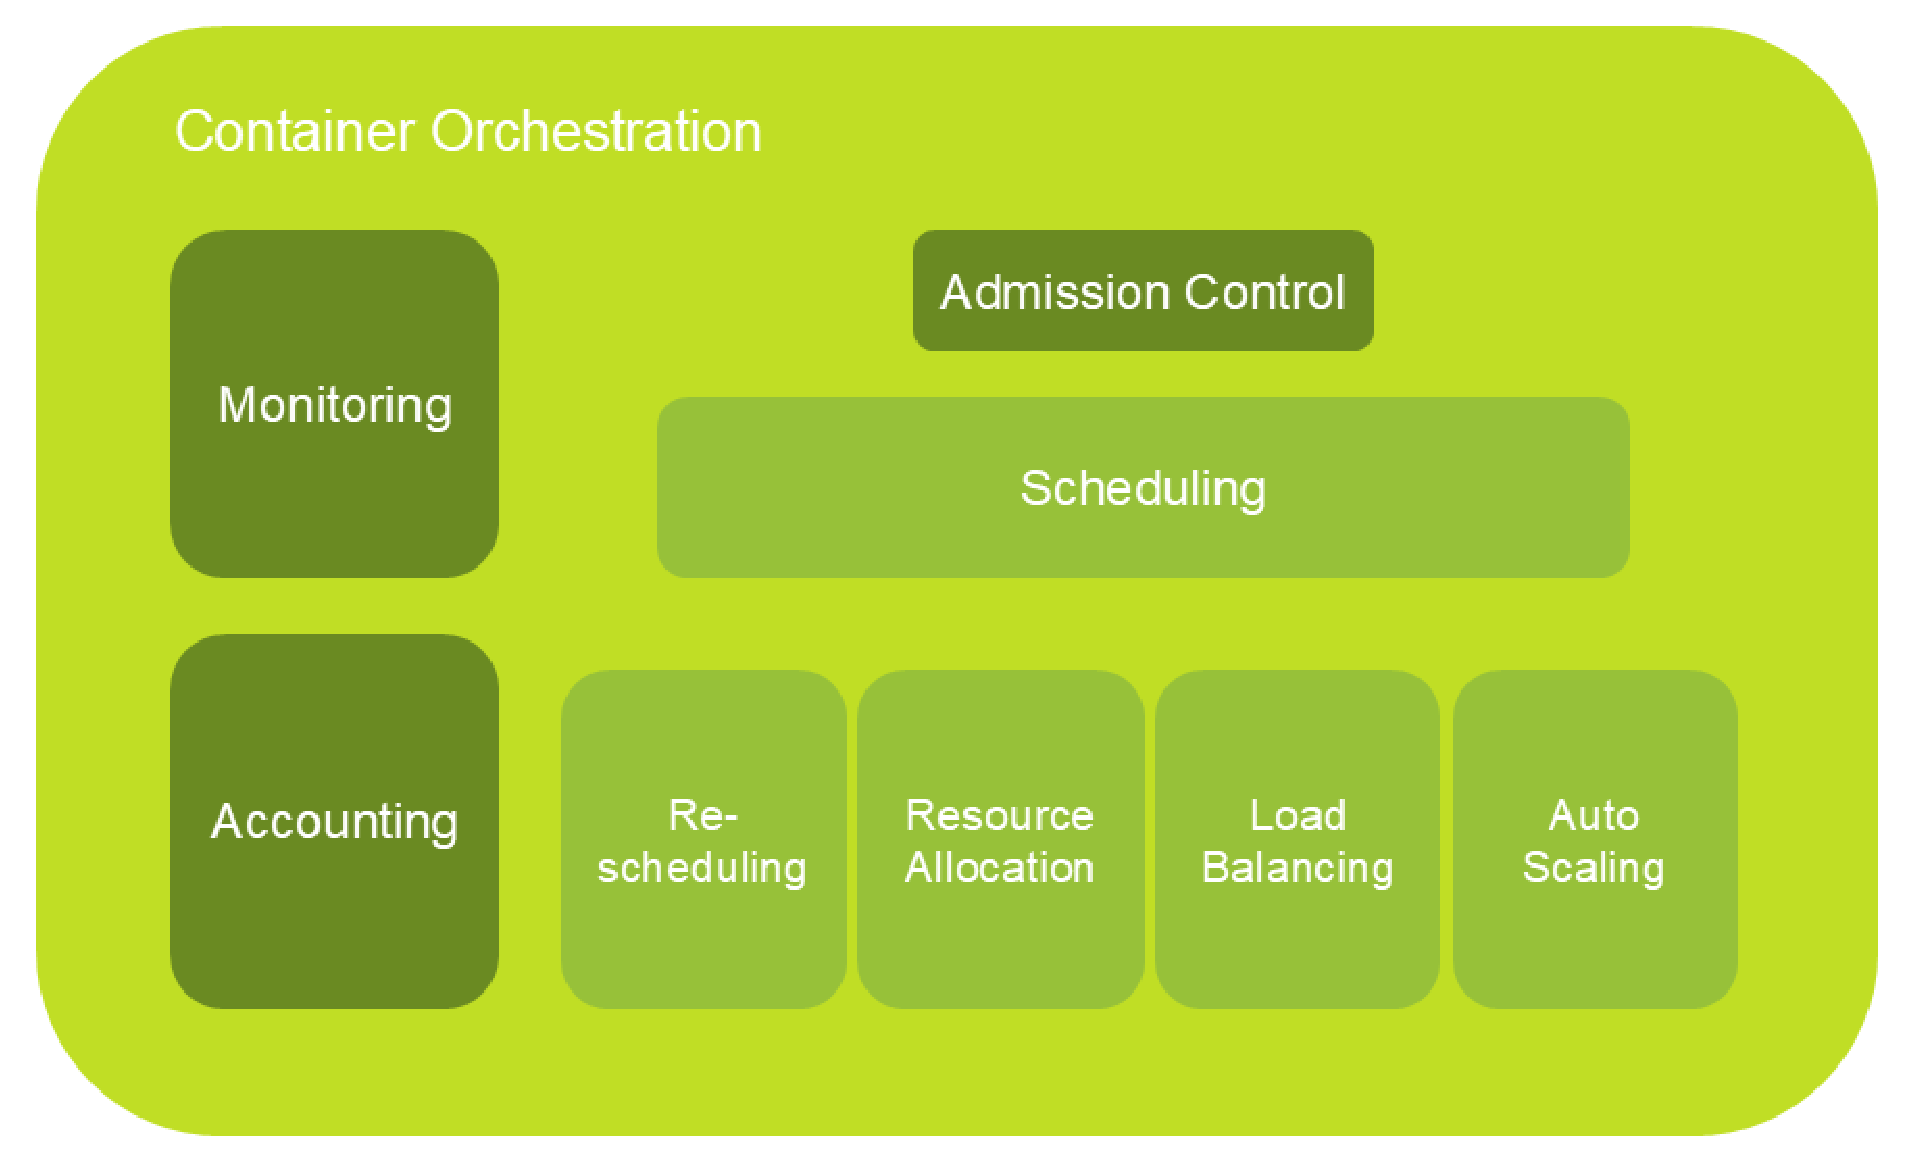
\includegraphics[width=0.8 \linewidth]{Thesis/Figures/Slide34.pdf}
\caption{\label{fig:Container Orchestration}Container Orchestration \cite{carrion2022Kubernetes}}
\end{figure}


\section{Best Practices for Designing Scalable Cloud-Native Architectures}

By integrating technologies like distributed tracing, chaos engineering and circuit breaking, cloud-native architectures can achieve high levels of scalability, flexibility and reliability. These practices allows organizations to fully leverage the advantages of cloud computing, ensuring their applications are resilient and capable of handling diverse and unpredictable workloads. \cite{r16}

\subsection{Distributed Tracing}

Distributed tracing is essential to understand how the requests flow through complex distributed systems \cite{r24}. It allows developers to track each requests as they passed through multiple microservices, facilitating the diagnosis of performance issues, pinpointing bottlenecks and enhancing application performance \cite{r25}. As shown in \autoref{fig:Distributed Tracing}, a service with a unique ID initiates a transaction by calling microservices A through E. Microservice A starts by invoking microservice B, which in turn calls microservices C and D, while A also calls microservice E, all of which are visualized as time spans to represent the complete trace of the request \cite{logz2024tracing}.

\clearpage

\captionsetup{justification=centering}
\begin{figure}[h]
\centering
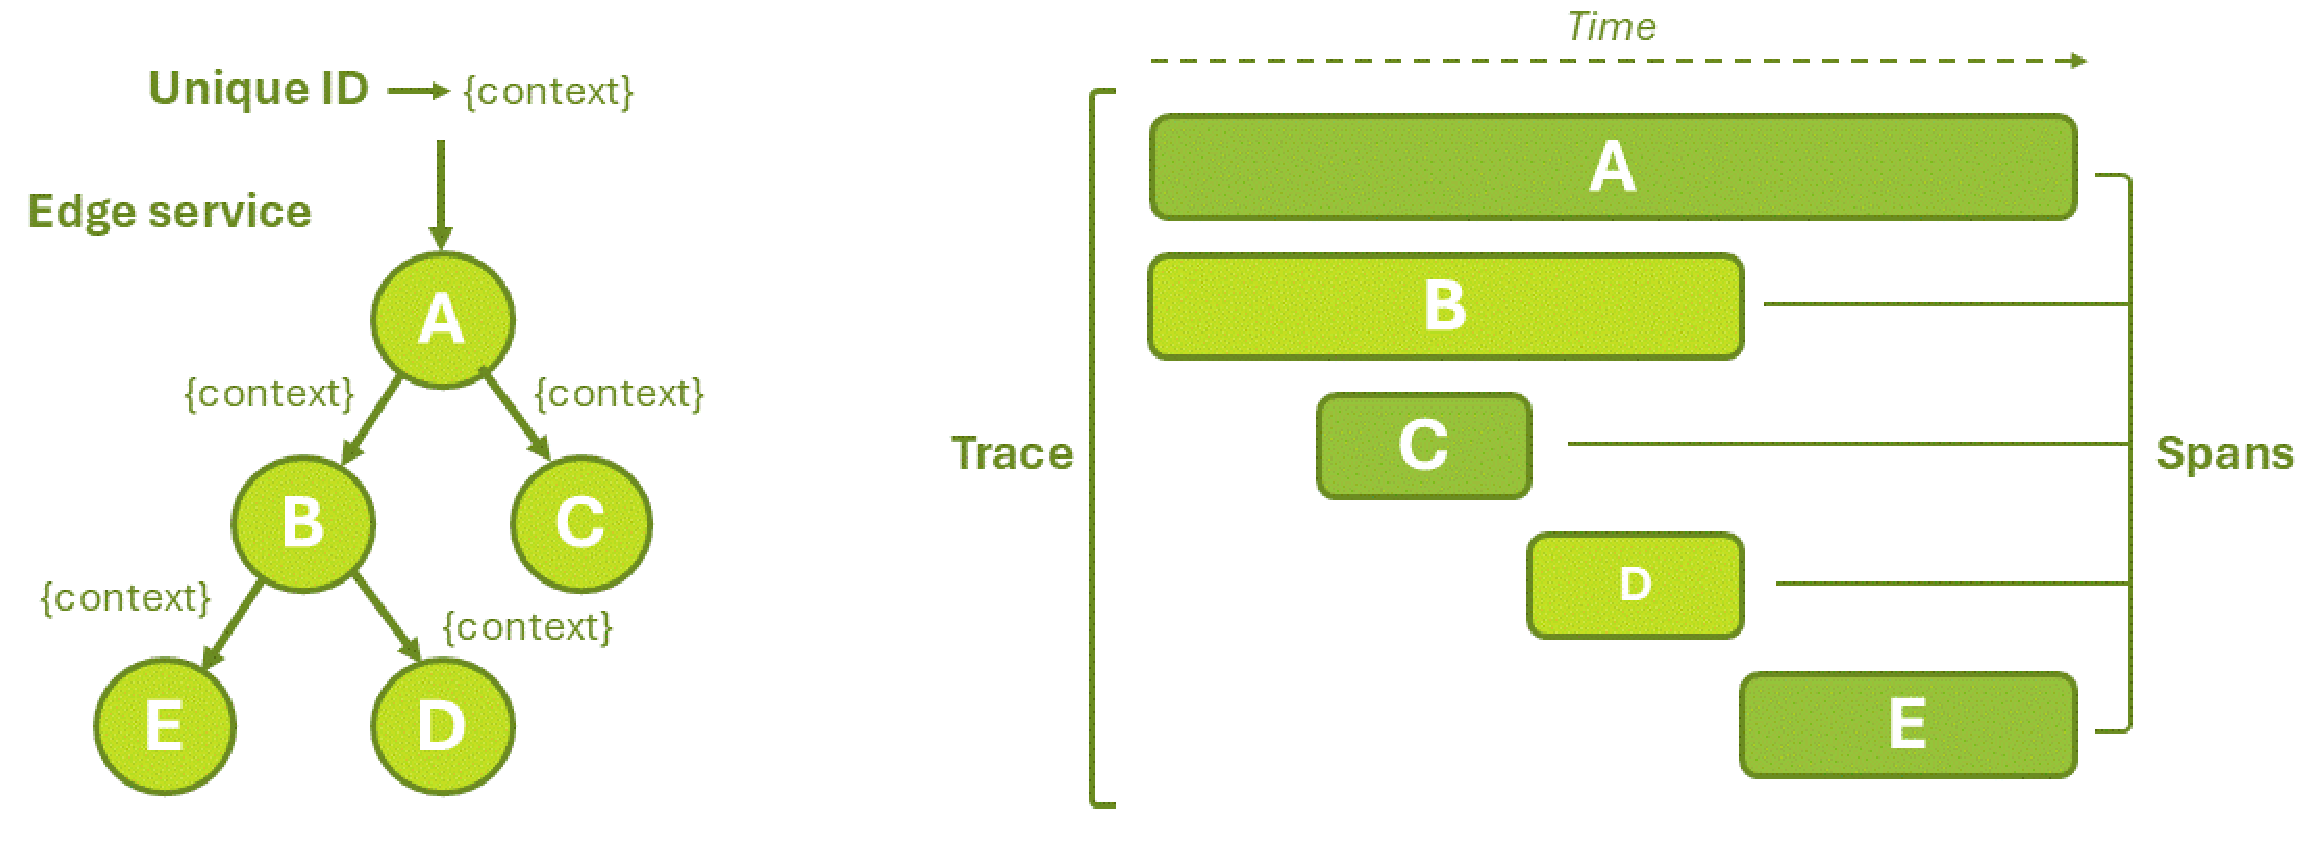
\includegraphics[width=1 \linewidth]{Thesis/Figures/Slide33.pdf}
\caption{\label{fig:Distributed Tracing}Distributed Tracing \cite{logz2024tracing}}
\end{figure}


\subsection{Circuit Breaking}


Circuit breaking is a technique that uses interceptors to check the health of services in terms of availability and responsiveness.The circuit breaker automatically rejects requests when a microservice is down, as shown in \autoref{fig:Circuit Breaker}. This prevents applications from waiting for a timeout due to service unavailability. This approach reduces application response time by eliminating unnecessary retries. When the service becomes available again, the circuit breaker automatically resets, allowing requests to pass through. To implement circuit breakers, all microservices must update and call each other using circuit breaker proxies. In addition, choosing appropriate timeout values for the circuit breaker can be challenging. Despite these trade-offs, circuit breakers are essential for maintaining and improving system responsiveness. \cite{r28}.


\captionsetup{justification=centering}
\begin{figure}[h]
\centering
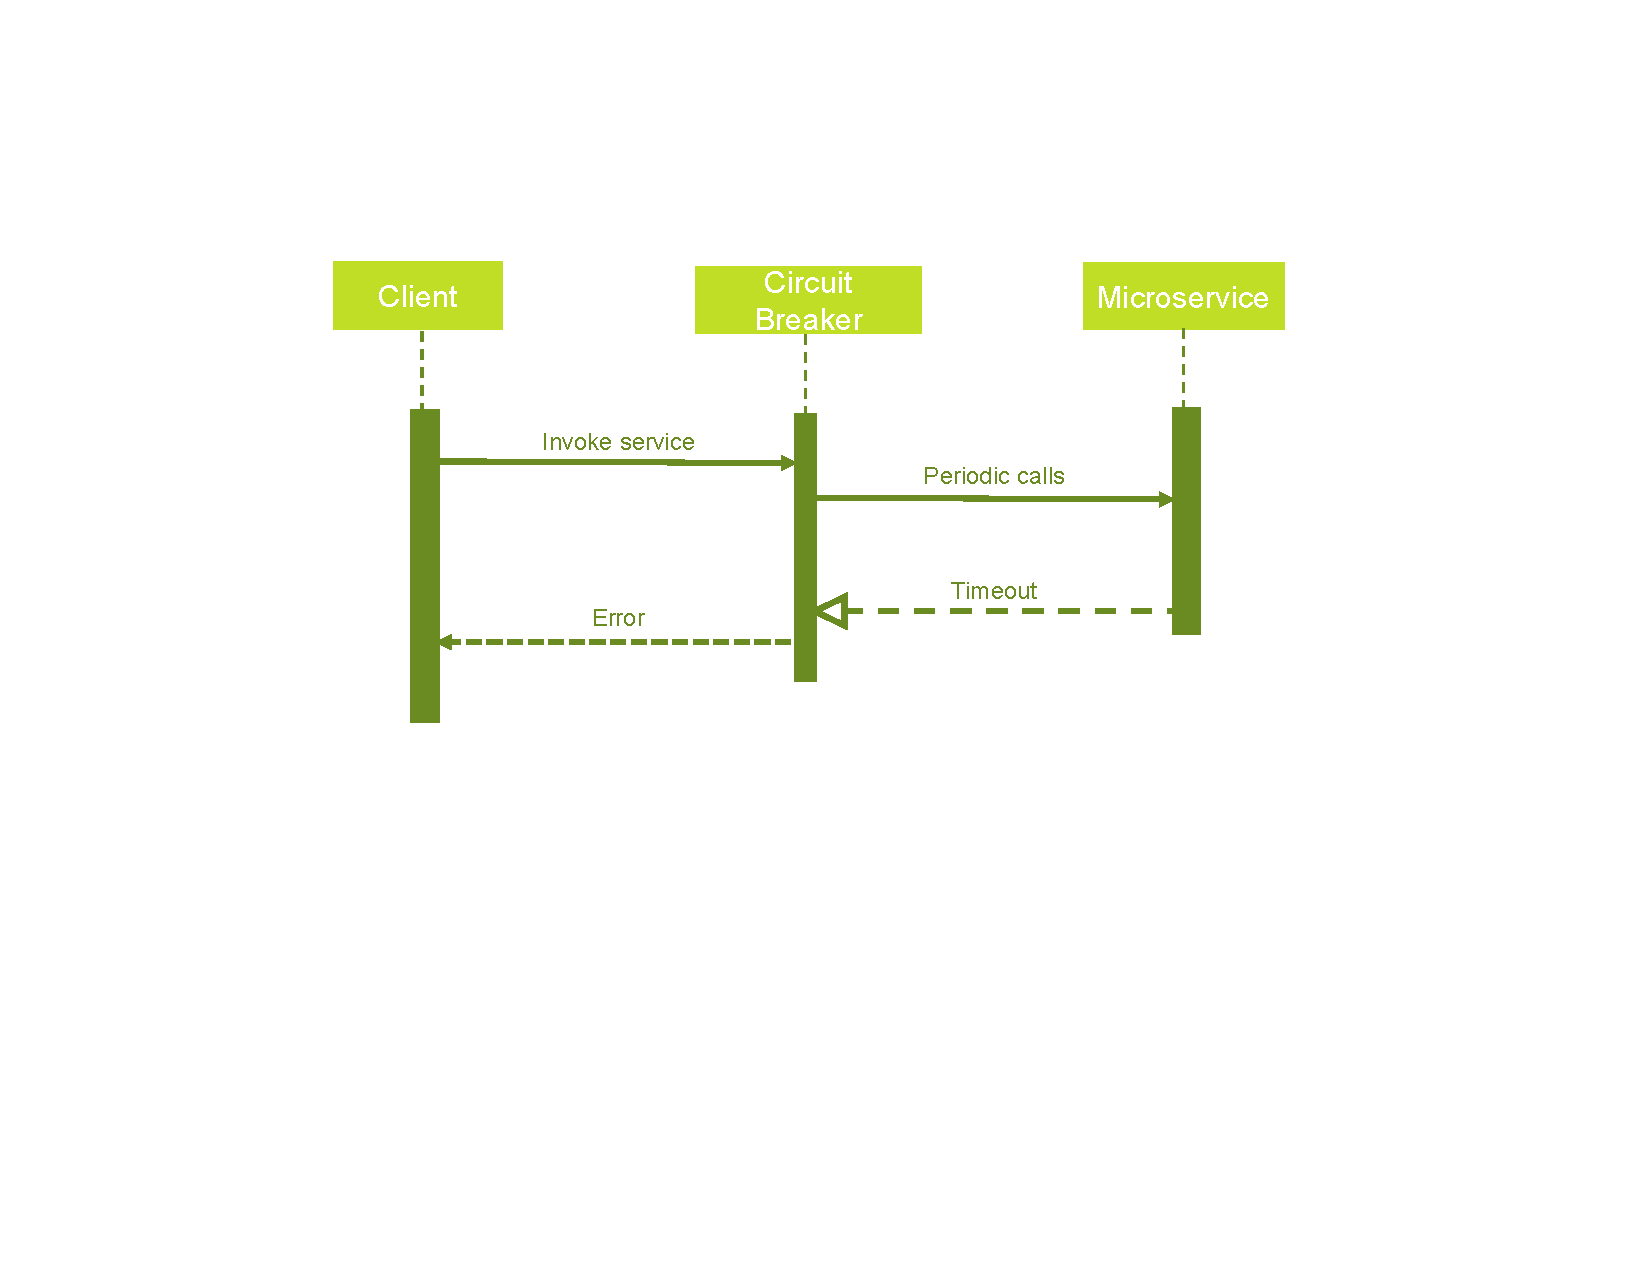
\includegraphics[width=1 \linewidth]{Thesis/Figures/Slide32.pdf}
\caption{\label{fig:Circuit Breaker}Circuit Breaker \cite{goyal2019circuit}}
\end{figure}


\subsection{Chaos Engineering}

The aim of chaos engineering is to test the resilience of distributed systems to determine how resilient they are. It involves simulation-based fault injection and is defined as "The discipline of experimenting on a distributed system to build confidence in the system's ability to withstand turbulent conditions in production". The basic idea behind chaos engineering is to deliberately subject the system to adverse conditions modelled on those that may occur in a real production environment. This method helps to identify any defects and provides insight into the resilience of the system. Organisations can proactively avoid such problems by identifying these vulnerabilities before they result in user problems. \cite{r29}

\section{Key Components of Cloud-Native Ecosystems}

This section examines the essential elements of cloud-native ecosystems, focusing on Kubernetes for container orchestration and resource autoscaling, as well as the tools and technologies required to secure and scale cloud-native architectures.

\subsection{Kubernetes}

Kubernetes is an open source container orchestration platform that automates the deployment, scaling and management of containerised applications. It provides a robust set of features, including a key-value pair store, API server, controller manager and scheduler, that streamline container operations and abstract the complexity of the underlying infrastructure, as shown in \autoref{fig:Kubernetes Architecture}. This abstraction allows developers to focus on building and deploying applications without worrying about the internal infrastructure. \cite{r32}

\captionsetup{justification=centering}
\begin{figure}[h]
\centering
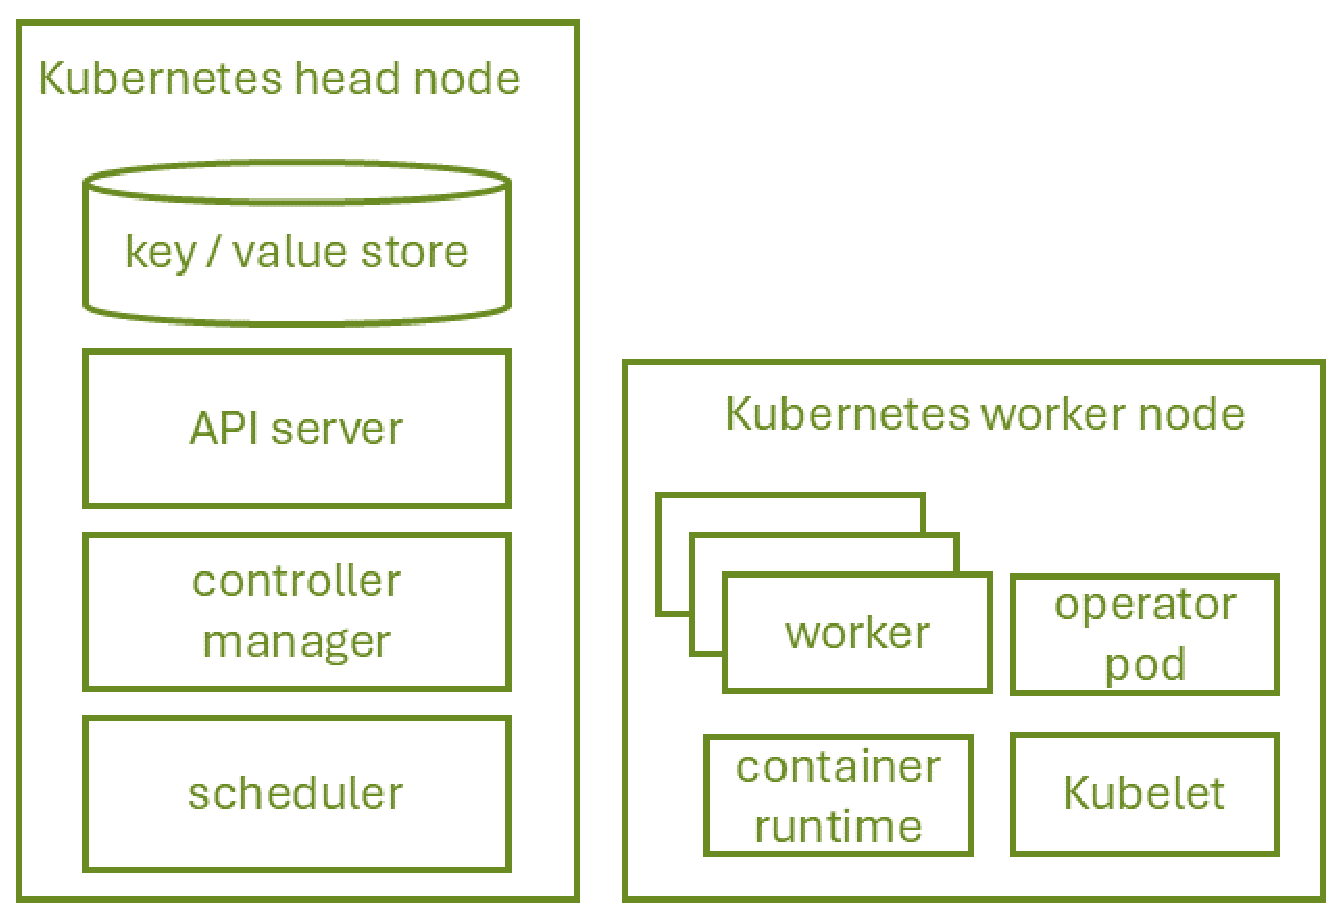
\includegraphics[width=0.8 \linewidth]{Thesis/Figures/Slide16.pdf}
\caption{\label{fig:Kubernetes Architecture}Kubernetes Architecture \cite{r34}}
\end{figure}

Kubernetes has become the de facto container management platform. It defines a declarative model for specifying a desired system state and implements controller logic that constantly strives to reconcile the actual system state with the desired state. The Kubernetes API server serves REST operations and provides the frontend to the clusters shared state. This state is stored in a key-value store. The values of these keys represent artifacts managed by Kubernetes, such as pods. Pods, which abstract containers, are the smallest deployable units in Kubernetes. Kubernetes manages the lifecycle of pods through various controllers, with the controller manager overseeing numerous controllers, such as the deployment and replica set controllers. For instance, the deployment controller continuously monitors the deployment manifest, which defines how replicated pods should be managed and ensures that the number of running pods matches the desired count in the cluster. \cite{r34}




\textbf{Minikube}


Minikube is a tool that allows developers to run Kubernetes clusters locally, providing a lightweight and easy to use solution for testing and developing Kubernetes applications. It creates a single node Kubernetes cluster within a virtual machine \abk{VM}{Virtual Machine} on a local system, providing an environment that closely simulates a Kubernetes cluster in production. This allows developers to experiment and test Kubernetes applications without having to deploy them to a full scale cloud-based cluster. To get started with Minikube, a few installation steps are required. First, it is necessary to install a hypervisor, which Minikube will use to create the VM. Next, kubectl the command-line tool for managing and interacting with Kubernetes clusters. After that, download and install the Minikube binary specific to the operating system, which simplifies the setup process by providing a single executable. Once everything is installed, you can start the Minikube cluster using the \texttt{minikube start} command. This command starts a local Kubernetes cluster, with Minikube automatically taking care of creating the VM, installing the Kubernetes components and configuring kubectl for use with the local cluster. \cite{sayfan2019hands}

\textbf{Kubectl}


Kubectl is a command-line tool used to interact with the Kubernetes control panel via the Kubernetes API. It allows users to perform various operations on Kubernetes resources. The config file contains kubectl configurations, which are located in the \texttt{\$HOME/.kube} directory, which can also be placed in other locations using the \texttt{KUBECONFIG} environment variable or the \texttt{kubeconfig} flag. The general syntax for using kubectl consists of four elements: command, type, name and flag. The command represents the operation you want to perform, such as creating, retrieving or deleting resources. The resource TYPE refers to the type of Kubernetes resource being managed, such as pod, service or deployment, which can be singular, plural or abbreviated. The NAME is the resource identifier, which is case-sensitive. If the name is omitted, kubectl will retrieve information for all resources of that type. In addition, flags allow you to customise commands by overriding defaults or environment variables. Kubectl also supports operations on multiple resources at once. You can either group resources of the same type, or specify different resource types individually. \cite{Kubernetes_doc}

\clearpage

\textbf{Helm}

Helm is a tool for managing Kubernetes packages, known as charts. A Helm chart is essentially a collection of files and information needed to deploy a Kubernetes application. Helm's purpose is to create charts from scratch, package them into \texttt{.tgz} files and store them in chart repositories or deploy them to Kubernetes clusters. Helm also manages the lifecycle of these charts, which includes installation, upgrades and uninstallation. There are three key components to Helm's structure a chart, a configuration and a release. A chart bundles all the resources needed to create an application, the config contains configuration settings that can be applied to the chart when creating a custom deployment and the release refers to a running instance of the chart combined with a specific configuration. Helm is divided into two primary components the Helm client and the Helm library. The Helm client is serve a command-line interface used by end users for tasks such as local chart development, repository management and release handling. On the other hand, Helm library, handles the core logic for operations like installing, upgrading, or uninstalling charts, while interfacing with the Kubernetes API server to provision resources. \cite{helm_docs}

\textbf{Kind}

Kind (Kubernetes in Docker) is a tool that allows users to create and manage local Kubernetes clusters using Docker containers. It's particularly useful for testing and development, providing a lightweight, easy way to spin up clusters without needing a full cloud-native environment. Kind works by running Kubernetes nodes inside Docker containers, simulating a full Kubernetes cluster. This makes it a preferred choice for local Kubernetes development, as it integrates well with existing Docker environments and simplifies the setup process. One of the key benefits of using Kind is its ability to create multi node clusters with minimal overhead. Developers can easily create clusters to test different Kubernetes features, workflows or applications on their local machines. Kind also inherits Docker's portability, allowing the same Kubernetes environment to be replicated across different machines. It supports most of the core Kubernetes features and can be integrated with continuous integration \abk{CI}{Continuous Integration} pipelines, making it a handy tool for automatically testing Kubernetes deployments during software development processes. However, because it's designed for local use, it lacks some of the scalability and performance optimisations found at the production level in Kubernetes clusters. Kind is a widely adopted solution in the Kubernetes ecosystem, particularly for developers who need a local Kubernetes environment for testing without the complexity of managing an actual Kubernetes infrastructure. \cite{kind_Kubernetes}


\subsection{Kubernetes Autoscaling}

Kubernetes autoscaling is used to control and manage the number of instances running in a cluster based on the load. This capability is necessary for sustaining efficient performance and expenditure in cloud-native applications. Kubernetes supports various types of autoscaling, including horizontal, vertical and cluster level autoscaling. horizontal pod autoscaling \abk{HPA}{Horizontal Pod Autoscaling} is used to increase the number of pods in deployment or replica set while vertical pod autoscaling \abk{VPA}{Vertical Pod Autoscaling} is used to change the container resource requirements. The process of scaling up or down the Kubernetes cluster is done by cluster autoscaler considering the usage of the pods. To achieve autoscaling in Kubernetes, there has to be creation of metrics and specifications of the parameters that should be crossed as the requirements for scaling. For example, the HPA uses metrics that come from the Kubernetes metrics server or any other custom metrics. If the defined metric proves to be higher than a set limit, the HPA will add more pod to help in handling the demand. On the other hand, if the usage goes below the set figure, the status will prescribe the number of pods to decrease. To achieve dynamic scaling, the loads that an application experiences are smoothed out and this makes the application adapt to changing loads on the system without the need for intervention thus increasing resource usage efficiency as well as decreasing the operational costs. \cite{Kubernetes_doc}


\textbf{Horizontal Pod Autoscaler}

HPA is one of the core components of Kubernetes that scales a deployment, a replica set, or a stateful set up or down depending on the observed central processing unit \abk{CPU}{Central Processing Unit} usage or other, user supplied metrics. Specifically, the primary goal of HPA is to make sure that the application can effectively respond to changes in load through the process of scaling out by creating more pods or scaling in by removing the unnecessary pods see \autoref{fig:Horizontal Pod Autoscaling}. HPA operates by constantly making a call to the Kubernetes metrics server to fetch the pods current utilization and then comparing it to the desired or target utilization from the HPA configuration. HPA configuration entails the identification of the target and a value below which a warning message should be generated. For instance, the specific goal of CPU utilization might be set at 70 percent. When the average CPU utilization of all pods in the deployment, HPA will scale up the pods, to spread the load evenly. On the other hand, if the present CPU usage is lesser than this indication, HPA will scale down the amount of pods. This process guarantees the responsiveness of the application in terms of internal and external loads, additionally it ensures efficiency in the use of resources. \cite{Kubernetes_doc}


\captionsetup{justification=centering}
\begin{figure}[h]
\centering
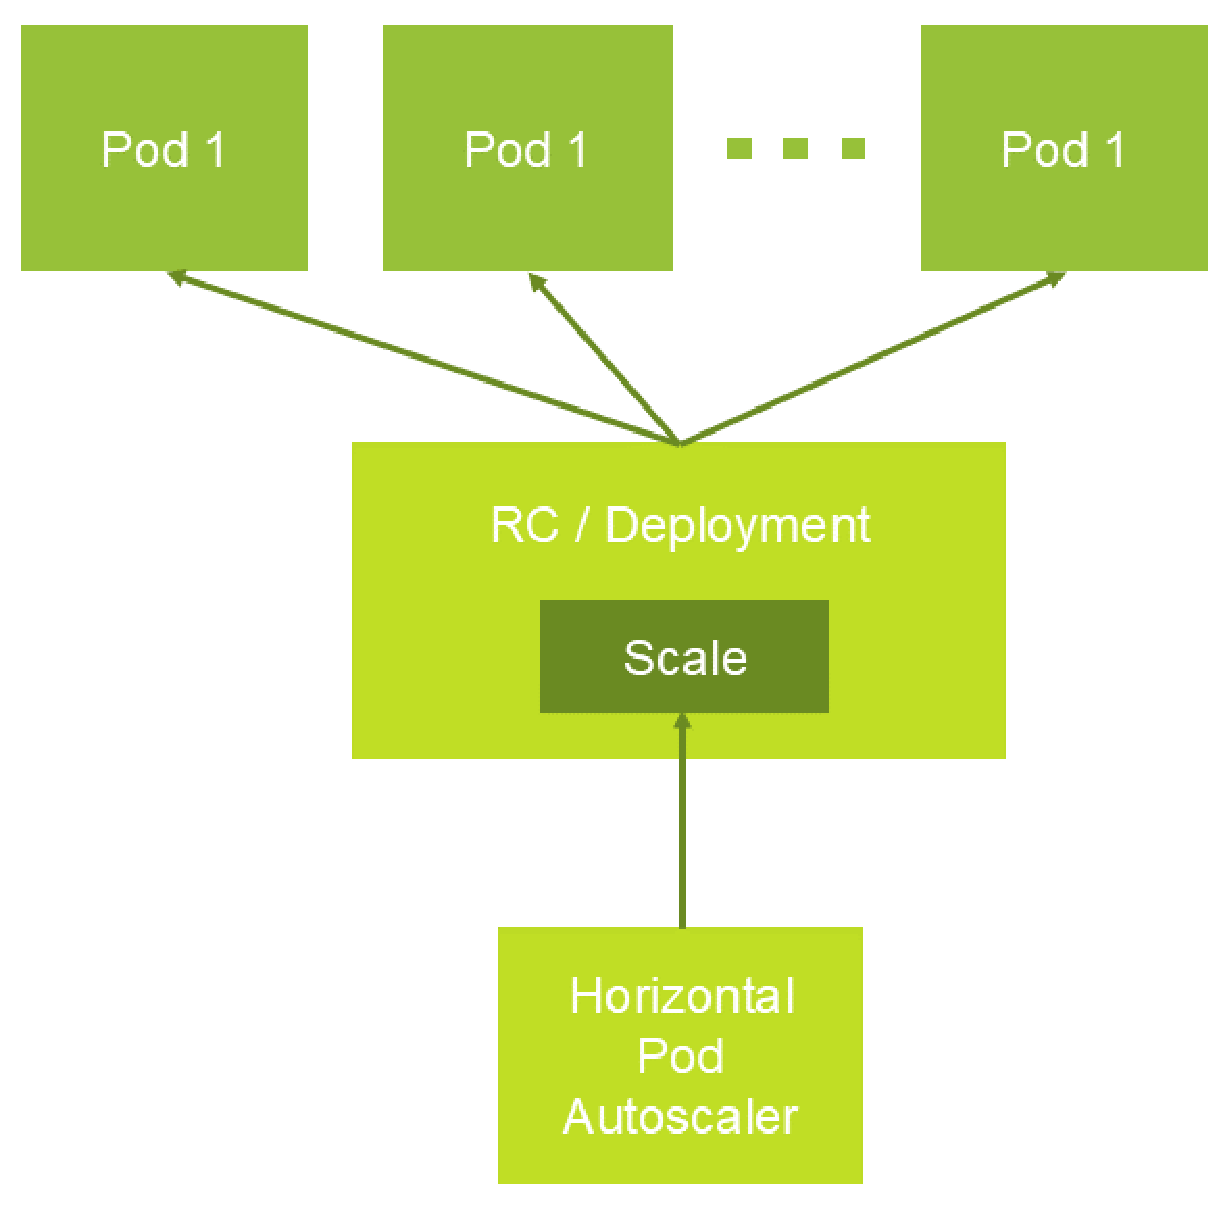
\includegraphics[width=0.6 \linewidth]{Thesis/Figures/Slide35.pdf}
\caption{\label{fig:Horizontal Pod Autoscaling}Horizontal Pod Autoscaling \cite{Kubernetes_doc}}
\end{figure}


\clearpage

\textbf{Vertical Pod Autoscaler}

VPA is another autoscaling feature in Kubernetes that focuses on adjusting the resource requests and limits for containers within a pod, rather than changing the number of pods as shown in \autoref{fig:Vertical Pod Autoscaling}. This autoscaling is very helpful for the applications with fluctuating demand in resources because with this approach the correct amount of CPU and RAM is allocated to each pod. VPA is always checking the resource utilization of pods and may give suggestions on increasing or decreasing the amount of resource provided or even making such changes on its own. \cite{vertical_pod_autoscaler}

\captionsetup{justification=centering}
\begin{figure}[h]
\centering
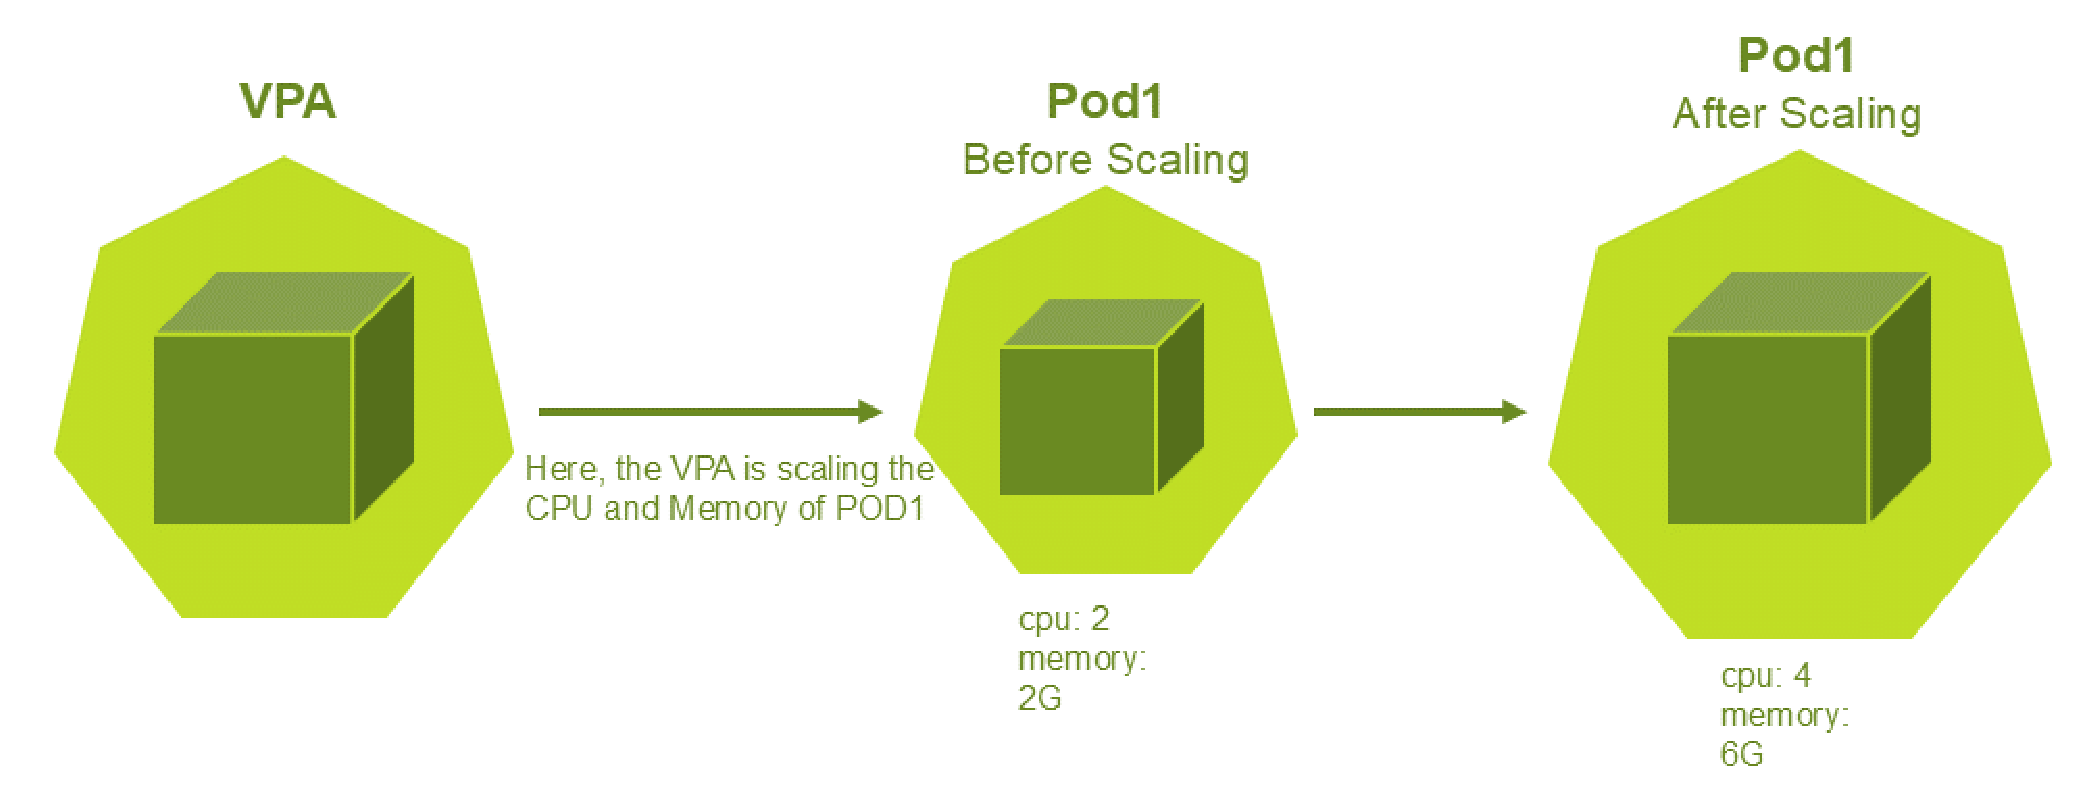
\includegraphics[width=1 \linewidth]{Thesis/Figures/Slide36.pdf}
\caption{\label{fig:Vertical Pod Autoscaling}Vertical Pod Autoscaling \cite{Kubernetes-vpa}}
\end{figure}

The VPA operates in three modes \texttt{Off}, \texttt{Auto} and \texttt{Recreate}. In \texttt{Off} mode, the VPA provides recommendations of changes that need to be made without actually making the changes. In \texttt{Auto} mode, which means that it optimizes them during the pod’s existence. \texttt{Recreate} mode entails restating the pod to make necessary changes on the available resource options. Still, this kind of flexibility is very useful to administrators because they can select a flow that is suitable for their application and the manner in which it will be run. In preventing wastage of resources, VPA assists in avoiding scenarios that may lead to performance throttle by ensuring that the value of pods converge towards the set limit, thus improving the stability of the Kubernetes applications. \cite{vertical_pod_autoscaler}




\section{Authentication and Authorization in Cloud-Native Architectures}

Authentication and authorization are critical to securing applications and services in cloud-native architectures. These architectures leverage the clouds inherent scalability, flexibility and distributed nature, necessitating modern, dynamic approaches to access control. Traditional security measures are often inadequate in such environments, where resources are highly distributed and dynamically scaled \cite{mohamed2024cloud}. Authentication involves verifying the identity of users or services, often implemented through techniques such as multi factor authentication \abk{MFA}{Multi Factor Authentication}, SSO and federated identity providers. SAML OAuth and OIDC are widely used standards that facilitate secure authentication and authorization, ensuring that users identities are verified and managed securely across various applications and services. \cite{r38, r39}

Authorization, on the other hand, determines the actions that authenticated users or services are allowed to perform only within a pod, rather than changing the number of pods as shown in \autoref{fig:Authentication and Authorization}. Cloud-native environments commonly employ RBAC and ABAC to manage permissions efficiently. RBAC assigns permissions to roles, simplifying management by grouping users into roles, based on their job functions, as seen in systems like Kubernetes \cite{r40}. ABAC, however, provides more granular control by using user attributes, resource types and environmental contexts to define access policies, thus allowing for dynamic and context aware access decisions \cite{r41}. Both methods are essential in ensuring that only authorized users can access specific resources, thereby enhancing security and operational efficiency in cloud-native architectures.

\captionsetup{justification=centering}
\begin{figure}[h]
\centering
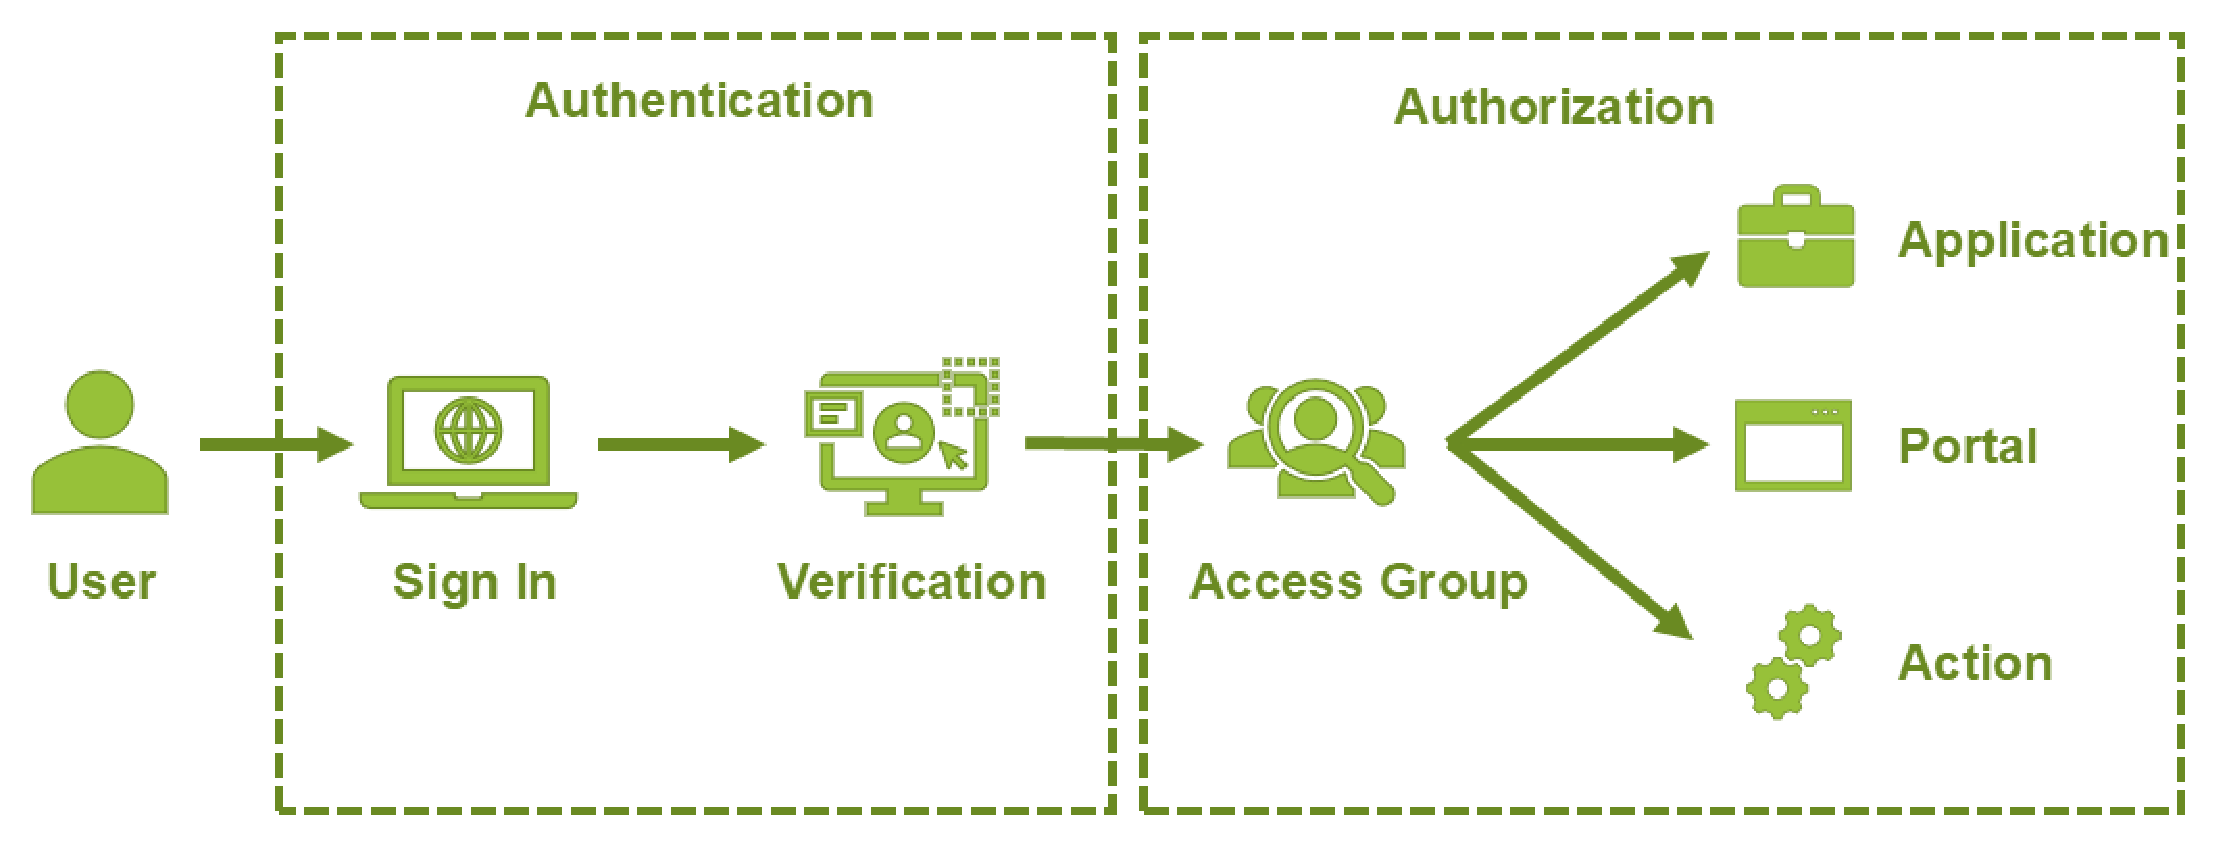
\includegraphics[width=1 \linewidth]{Thesis/Figures/Slide7.pdf}
\caption{\label{fig:Authentication and Authorization}Authentication and Authorization Flow \cite{r42}}
\end{figure}

\subsection{Keycloak for Authentication}

Keycloak is an open source identity and access management \abk{IAM}{Identity and Access Management} solution that provides a comprehensive approach for authentication in cloud-native architectures. The process begins when the client passes user data to Keycloak for authentication. After successful authentication, the application receives the access and ID tokens see \autoref{fig:Authentication}. Keycloak supports a wide range of authentication mechanisms, including multi-factor authentication MFA, SSO and social login, integrating seamlessly with modern applications and services. Keycloak simplifies the process of securing applications by providing built-in support for standards such as OAuth 2.0, OpenID Connect and SAML 2.0, which are crucial for verifying user identities and managing access across distributed systems. \cite{r38}

One of the primary advantages of Keycloak is its ability to act as a centralized authentication server, offering a single point of management for user identities and credentials. This centralized approach enhances security by enabling consistent application of authentication policies and reducing the complexity of managing credentials across multiple services. Keycloak also supports federated identity providers, allowing users to authenticate using their existing accounts from platforms like Google, Facebook and Microsoft Azure AD. This flexibility not only improves user experience by simplifying login processes but also strengthens security through robust identity verification methods \cite{keycloak_doc}. Moreover, Keycloak provides an intuitive administrative console for managing users, roles and permissions, making it easier for administrators to implement and enforce security policies across their cloud-native environments.


\captionsetup{justification=centering}
\begin{figure}[h]
\centering
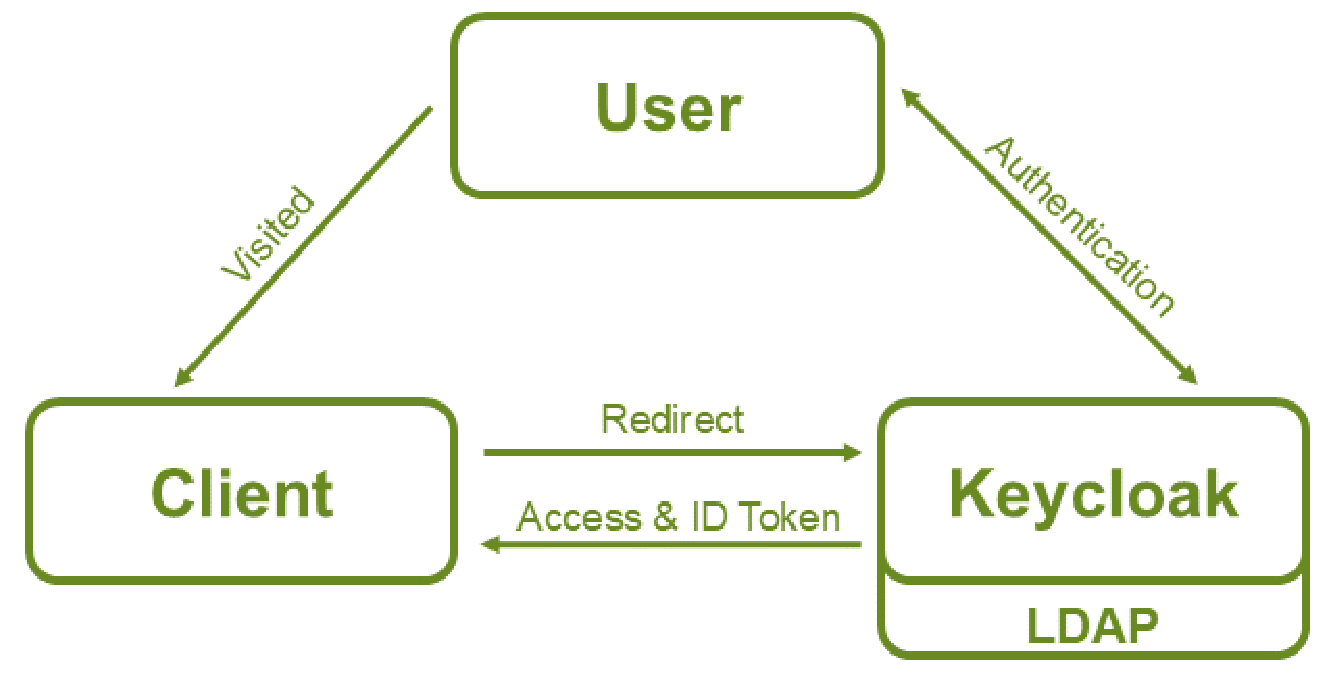
\includegraphics[width=0.65 \linewidth]{Thesis/Figures/Slide5.pdf}
\caption{\label{fig:Authentication}Keycloak Authentication Flow \cite{r45}}
\end{figure}



\textbf{Security Assertion Markup Language}

Security assertion markup language \abk{SAML}{Security Assertion Markup Language} is an open standard that uses XML encoding for security assertions and SAML messages as captured by the SAML specifications. It supports protocol bindings, which can be thought of as the insertion of SAML constructs into different transport layers, such as simple object access protocol \abk{SOAP}{Simple Object Access Protocol} over hypertext transfer protocol \abk{HTTP}{Hypertext Transfer Protocol}. In addition to profiles, SAML also describes in detail how a SAML assertion should be used in a communication protocol and also details security considerations when using SAML in different applications. An example is the artifact profile that ensures SSO of a user with a browser, a source site and a target site. In this protocol, there is a user who has already authenticated to the source site and returns, possibly by redirecting to the target site. The source site, which identifies the user's browser, stores the user's identity credential and sends the browser with the stored credential an identity credential and a SAML artifact, which is a reference to the stored credential, to the target site. When this artifact is received, the target site requests an assertion from the source site, which then verifies the user's authentication by providing the assertion to the target site, as shown in \autoref{fig:Security Assertion Markup Language (SAML)}. \cite{gross2003security}



\captionsetup{justification=centering}
\begin{figure}[h]
\centering
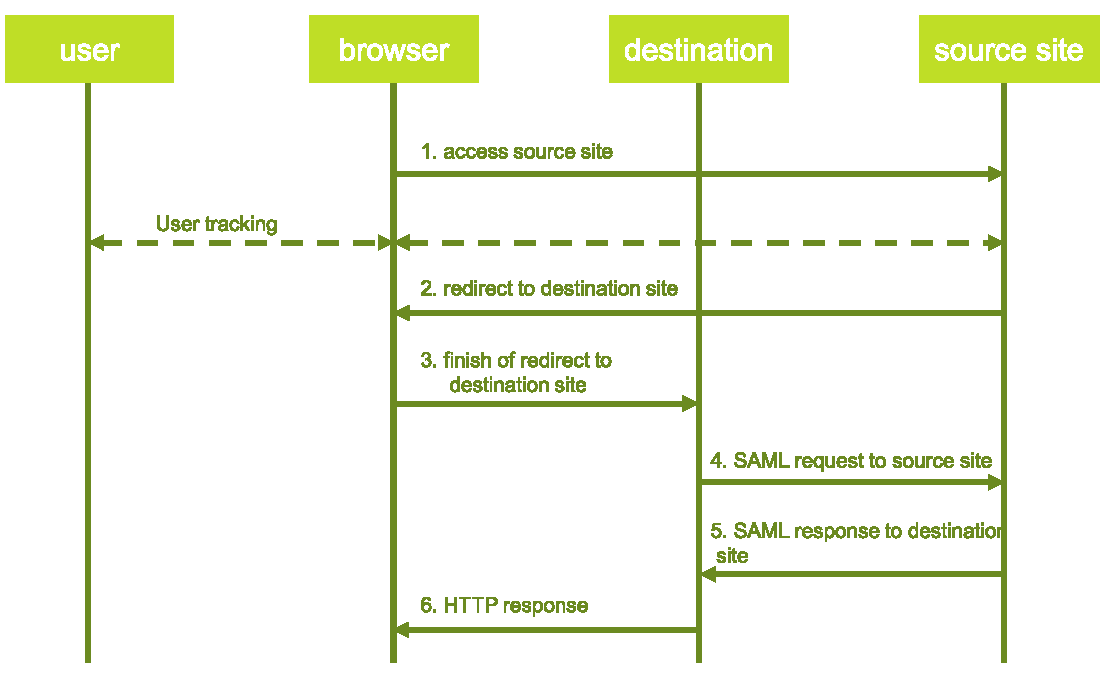
\includegraphics[width=0.75 \linewidth]{Thesis/Figures/Slide37.pdf}
\caption{\label{fig:Security Assertion Markup Language (SAML)}Authentication Flow of SAML \cite{gross2003security}}
\end{figure}

\clearpage

\textbf{Open Authorization}

Open Authorization \abk{OAuth}{Open Authorization} is an open standard that provides an efficient mechanism for users to use APIs in a standardized and secure way. The system allows users, known as resource owners, to allow third party applications, known as clients, to interact with their online resources on their behalf without having to share their credentials. The OAuth protocol consists of four primary components The resource server, which hosts the user's data. The client, which requests access to protected content from the resource server on behalf of the user and the authorization server, which authenticates the user and returns tokens that act as credentials for the client to access the resource server. In addition, the OAuth protocol allows end users to specify the level of access granted to applications, ensuring that only authorised applications can perform the required tasks. The authorization code flow is a key OAuth flow, often used for server side applications with a back-end server. In this flow, the client initiates an authorisation request by redirecting the user to the authorization server, which performs an authentication process and prompts the user for consent to grant access. Once the user has agreed, the authorisation server sends the required authorisation code back to the client via the user's browser or mobile application. The client then exchanges the code with the authorisation server in return for an access token, which is then used to access the relevant data held by the resource server on behalf of the user, as shown in \autoref{fig:OAuth 2.0}. This flow provides enhanced security by ensuring that access tokens are not exposed directly to the user but are securely handled by the clients backend server. The use of the authorization code flow facilitates secure and controlled access to user data across a broad spectrum of applications and platforms in accordance with the standards set out by OAuth. \cite{ranjbar2012authentication}
 

\captionsetup{justification=centering}
\begin{figure}[h]
\centering
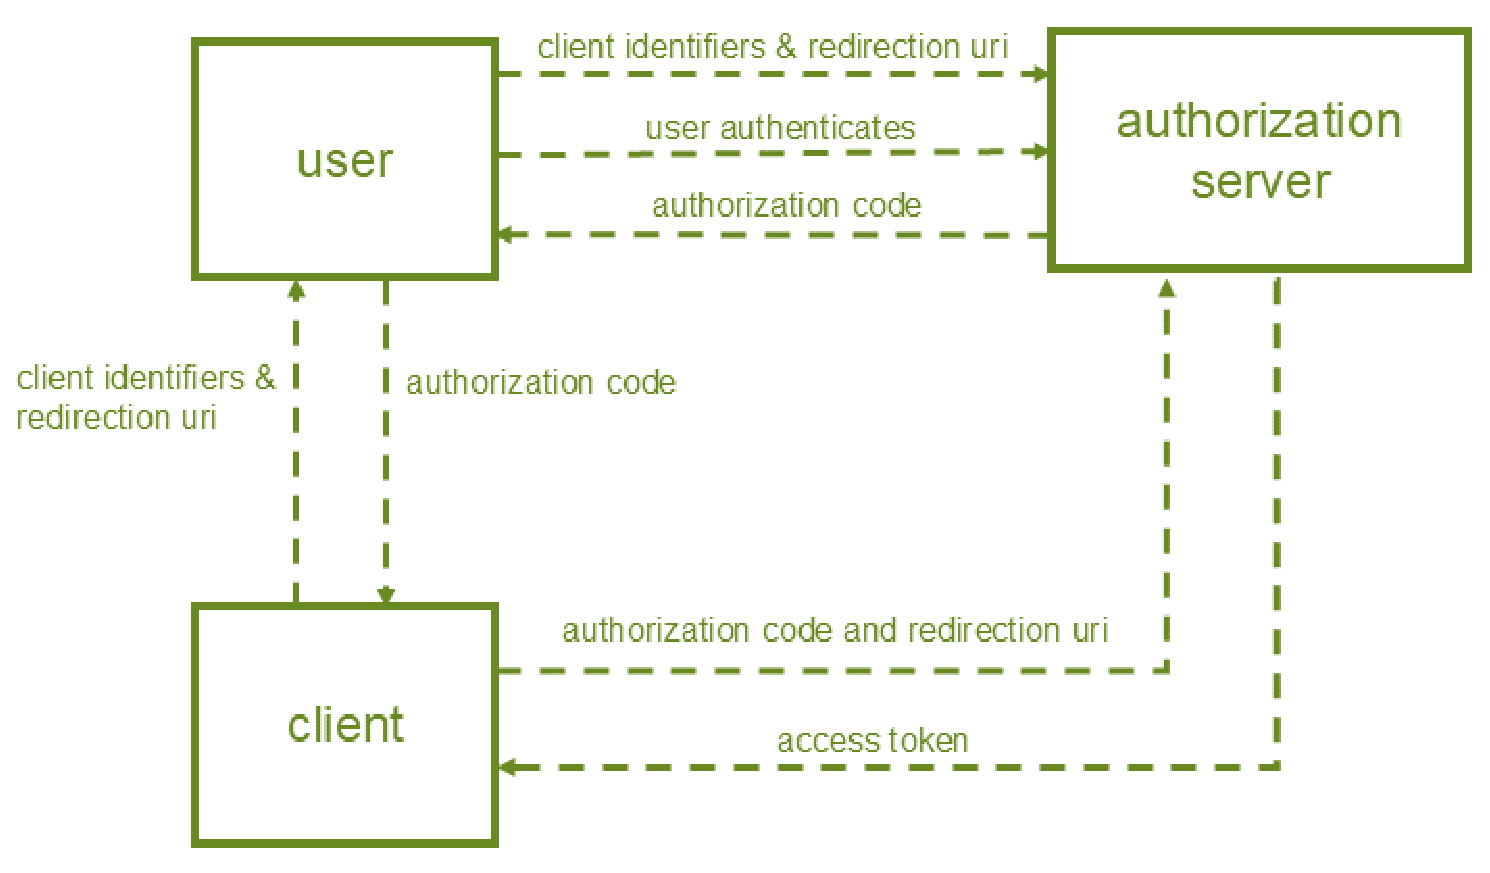
\includegraphics[width=1 \linewidth]{Thesis/Figures/Slide39.pdf}
\caption{\label{fig:OAuth 2.0}OAuth Authorization Flow \cite{ranjbar2012authentication}}
\end{figure}

\clearpage

\textbf{OpenID Connect}

OpenID Connect is a simple identity layer built on top of the OAuth 2.0 protocol that allows clients to verify the identity of end users based on authentication performed by an authorization server, also called an OpenID provider. It extends OAuth 2.0 by using authentication requests that include the OpenID scope, allowing the OpenID provider to issue ID tokens in the form of JSON web tokens \abk{JWT}{JSON Web Tokens} that contain information about the user's authentication. The protocol follows a flow where the client sends an authentication request to the OpenID provider, the OpenID provider verifies the end user and grants the permission. An access token is then returned by the OpenID provider. The client can use the access token to request additional information about the end user from the OpenID provider's UserInfo endpoint. The endpoint responds with user profile information. OpenID Connect thus extends OAuth 2.0 by adding a standardised way of providing authentication and identity information, making it interoperable and suitable for a wide range of web, mobile and API based applications. \autoref{fig:OIDC} shows the complete authentication protocol flow. \cite{openid-connect-core-1_0}


\captionsetup{justification=centering}
\begin{figure}[h]
\centering
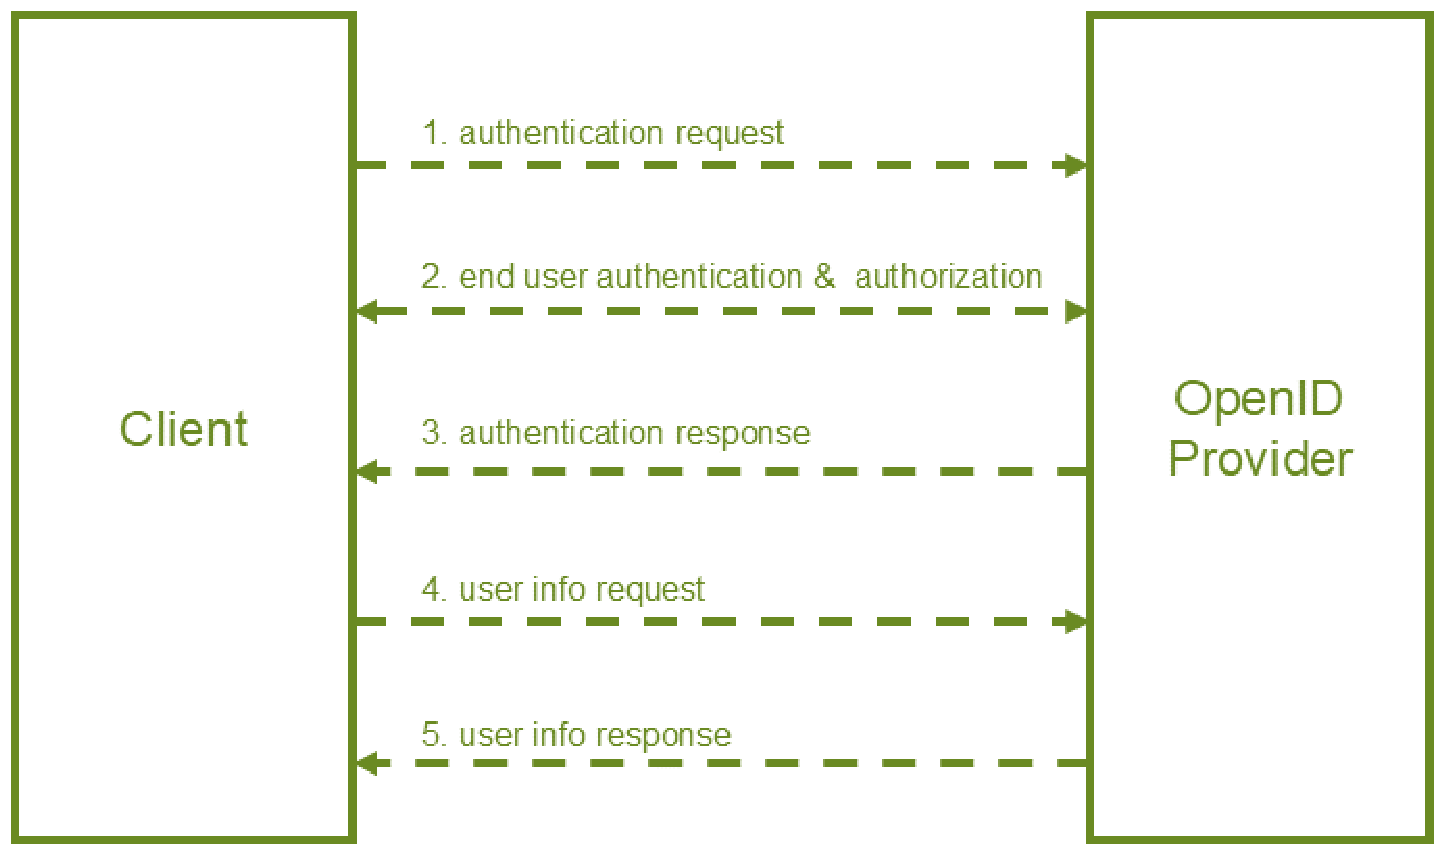
\includegraphics[width=0.9 \linewidth]{Thesis/Figures/Slide38.pdf}
\caption{\label{fig:OIDC}OpenID Connect Protocol \cite{openid-connect-core-1_0}}
\end{figure}

\subsection{Kubernetes Role-Based Access Control for Authorization}

RBAC is a comprehensive mechanism for managing authorization in cloud-native environments. It allows administrators to define and enforce policies using config files that dictate what actions users and services can perform within a Kubernetes cluster as shown in \autoref{fig:Authorization}. RBAC achieves this by assigning roles to users, groups, or service accounts and then binding these roles to specific permissions. This model simplifies the management of access control by organizing permissions based on roles rather than individual users, which is particularly beneficial in large and dynamic environments like those managed by Kubernetes. \cite{r40}
\clearpage

\captionsetup{justification=centering}
\begin{figure}[h]
\centering
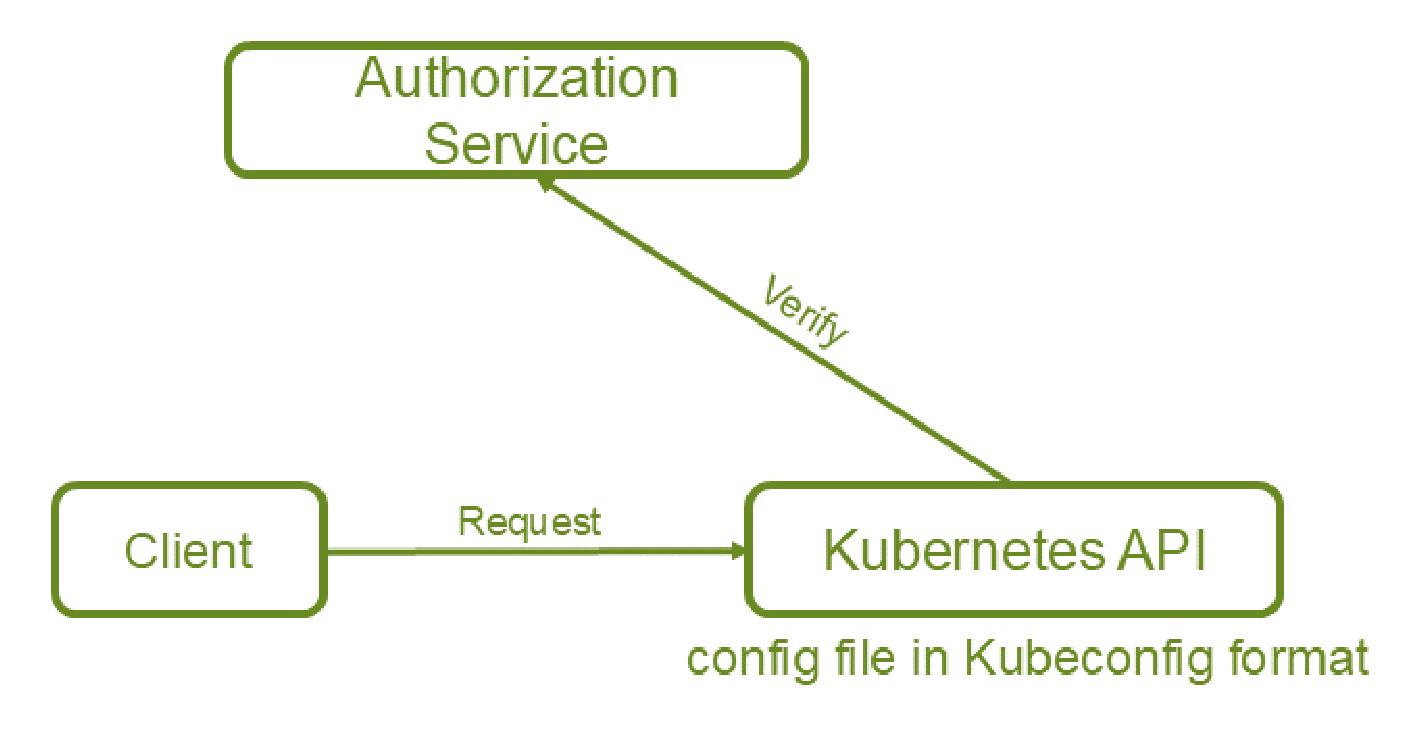
\includegraphics[width=0.7 \linewidth]{Thesis/Figures/Slide6.pdf}
\caption{\label{fig:Authorization}Authorization Request Flow \cite{r47}}
\end{figure}


\textbf{Components of Role-based Access Control:}

Roles, RoleBindings, ClusterRoles and ClusterRoleBindings are four components of RBAC. Roles and RoleBindings are namespace scoped allowing for fine-grained control over resources within the specific namespaces. ClusterRoles and ClusterRoleBindings on the other hand are cluster scoped allowing administrators to define global permissions that apply across all namespaces. This flexibility allows for precise and scalable access control management. By leveraging RBAC, organizations can ensure that users and services operate with the principle of least privilege, enhancing the security and stability of their cloud-native applications. Additionally, Kubernetes RBAC integrates seamlessly with other authentication mechanisms, such as OAuth 2.0 and OIDC , providing a comprehensive security solution that covers both authentication and authorization. \cite{Kubernetes_doc}

\textbf{User Accounts}

In Kubernetes, user accounts are identities assigned to human users, such as administrators, developers, or other team members, who need to access the Kubernetes cluster to perform tasks like development, maintenance, or administrative operations. These user accounts are managed outside of Kubernetes, typically by an identity provider and are used to authenticate and authorize access to the cluster resources. RBAC policies are applied to these user accounts to define what actions they can perform within the cluster, ensuring that access is restricted based on roles and responsibilities. \cite{rahasak_Kubernetes_rbac}


\textbf{Service Accounts}

Service accounts are identities specifically designed for software resources and processes that run within the Kubernetes environment. Unlike user accounts, service accounts are used by applications and processes, such as pods, to authenticate with the Kubernetes API server. Each namespace in Kubernetes comes with a default service account, which is automatically assigned to pods unless a different service account is specified. However, this default service account has minimal permissions. To grant more specific permissions or to have finer control over what an application or process can do within the cluster, custom service accounts can be created and managed using RBAC policies, allowing secure and restricted access for the applications running in the Kubernetes environment. \cite{rahasak_Kubernetes_rbac}

\clearpage

\textbf{Role}

A role in Kubernetes is a namespaced resource that defines a set of permissions specific to a particular namespace. When you create a role, you need to specify the namespace it belongs to, as its permissions are limited to that namespace only. Roles are used to grant access to resources such as pods, services or config maps within a particular namespace. For example, a role might only allow a user or service account to read, watch and list pods within the default namespace. This is achieved by defining the permissions in a role configuration. In the \autoref{listingsnippet:1} code snippet, the Role named \texttt{pod-reader} grants read-only access to pods in the \texttt{default} namespace. The rules section specifies that the role will allow the get, watch and list actions to be performed on pods, but only within this particular namespace. \cite{Kubernetes_doc}


\listingsnippet{Role Example \cite{Kubernetes_doc}}{

\vspace{0.3cm}

\hspace{0.25cm} \texttt{apiVersion: rbac.authorization.k8s.io/v1}

\hspace{0.25cm} \texttt{kind: Role}

\vspace{0.3cm}

\hspace{0.25cm} \texttt{metadata:}

\hspace{1cm} \texttt{namespace: default}

\hspace{1cm}name: \texttt{pod-reader}

\vspace{0.3cm}

\hspace{0.25cm} \texttt{rules:}

\hspace{0.25cm} \texttt{- apiGroups: [""]}

\hspace{1cm}  \texttt{resources: ["pods"]}
  
\hspace{1cm}  \texttt{verbs: ["get", "watch", "list"]}

\vspace{0.3cm}

}


\textbf{ClusterRole}

In Kubernetes, the ClusterRole is a non-namespaced resource, meaning it has cluster wide scope. ClusterRoles are more versatile than Roles because they can define permissions not only for cluster scoped resources, such as nodes, but also for namespaced resources across all namespaces. ClusterRoles can be used to grant broad permissions, such as reading secrets in any namespace or accessing non resource 
\abk{URL}{Uniform Resource Locator}. For instance, the following ClusterRole configuration grants read access to secrets across all namespaces. In code snippet \autoref{listingsnippet:2}, the ClusterRole named \texttt{secret-reader} allows the get, watch and list actions on secrets, enabling the user or Service Account to read secrets in any namespace. Since ClusterRoles are cluster scoped, they provide a more flexible and powerful way to manage permissions across the entire Kubernetes cluster. \cite{Kubernetes_doc}

\listingsnippet{ClusterRole Example \cite{Kubernetes_doc}}{

\vspace{0.3cm}

\hspace{0.25cm} \texttt{apiVersion: rbac.authorization.k8s.io/v1}

\vspace{0.3cm}

\hspace{0.25cm} \texttt{kind: ClusterRole}

\vspace{0.3cm}

\hspace{0.25cm} \texttt{metadata:}

\hspace{1cm}\texttt{name: secret-reader}

\vspace{0.3cm}

\hspace{0.25cm} \texttt{rules:}

\hspace{0.25cm} \texttt{- apiGroups: [""]}

\hspace{1cm}\texttt{resources: ["secrets"]}

\hspace{1cm}\texttt{verbs: ["get", "watch", "list"]}

\vspace{0.3cm}
}

\textbf{RoleBinding}

A RoleBinding in Kubernetes is used to associate a Role with one or more users, groups, or service accounts within a specific namespace. This means that the permissions defined in the Role are granted to the specified subjects, but only within the namespace where the RoleBinding is created. For example, you might have a RoleBinding that grants a \texttt{pod-reader} role to a user in the namespace named \texttt{namespace1}, allowing her to read pod information only in that namespace as shown in the \autoref{fig:RoleBinding}. RoleBindings can also reference ClusterRoles to apply cluster scoped permissions to resources within a single namespace. This flexibility allows administrators to define common roles across the cluster and then apply them in different namespaces using RoleBindings. \cite{Kubernetes_doc}



\captionsetup{justification=centering}
\begin{figure}[h]
\centering
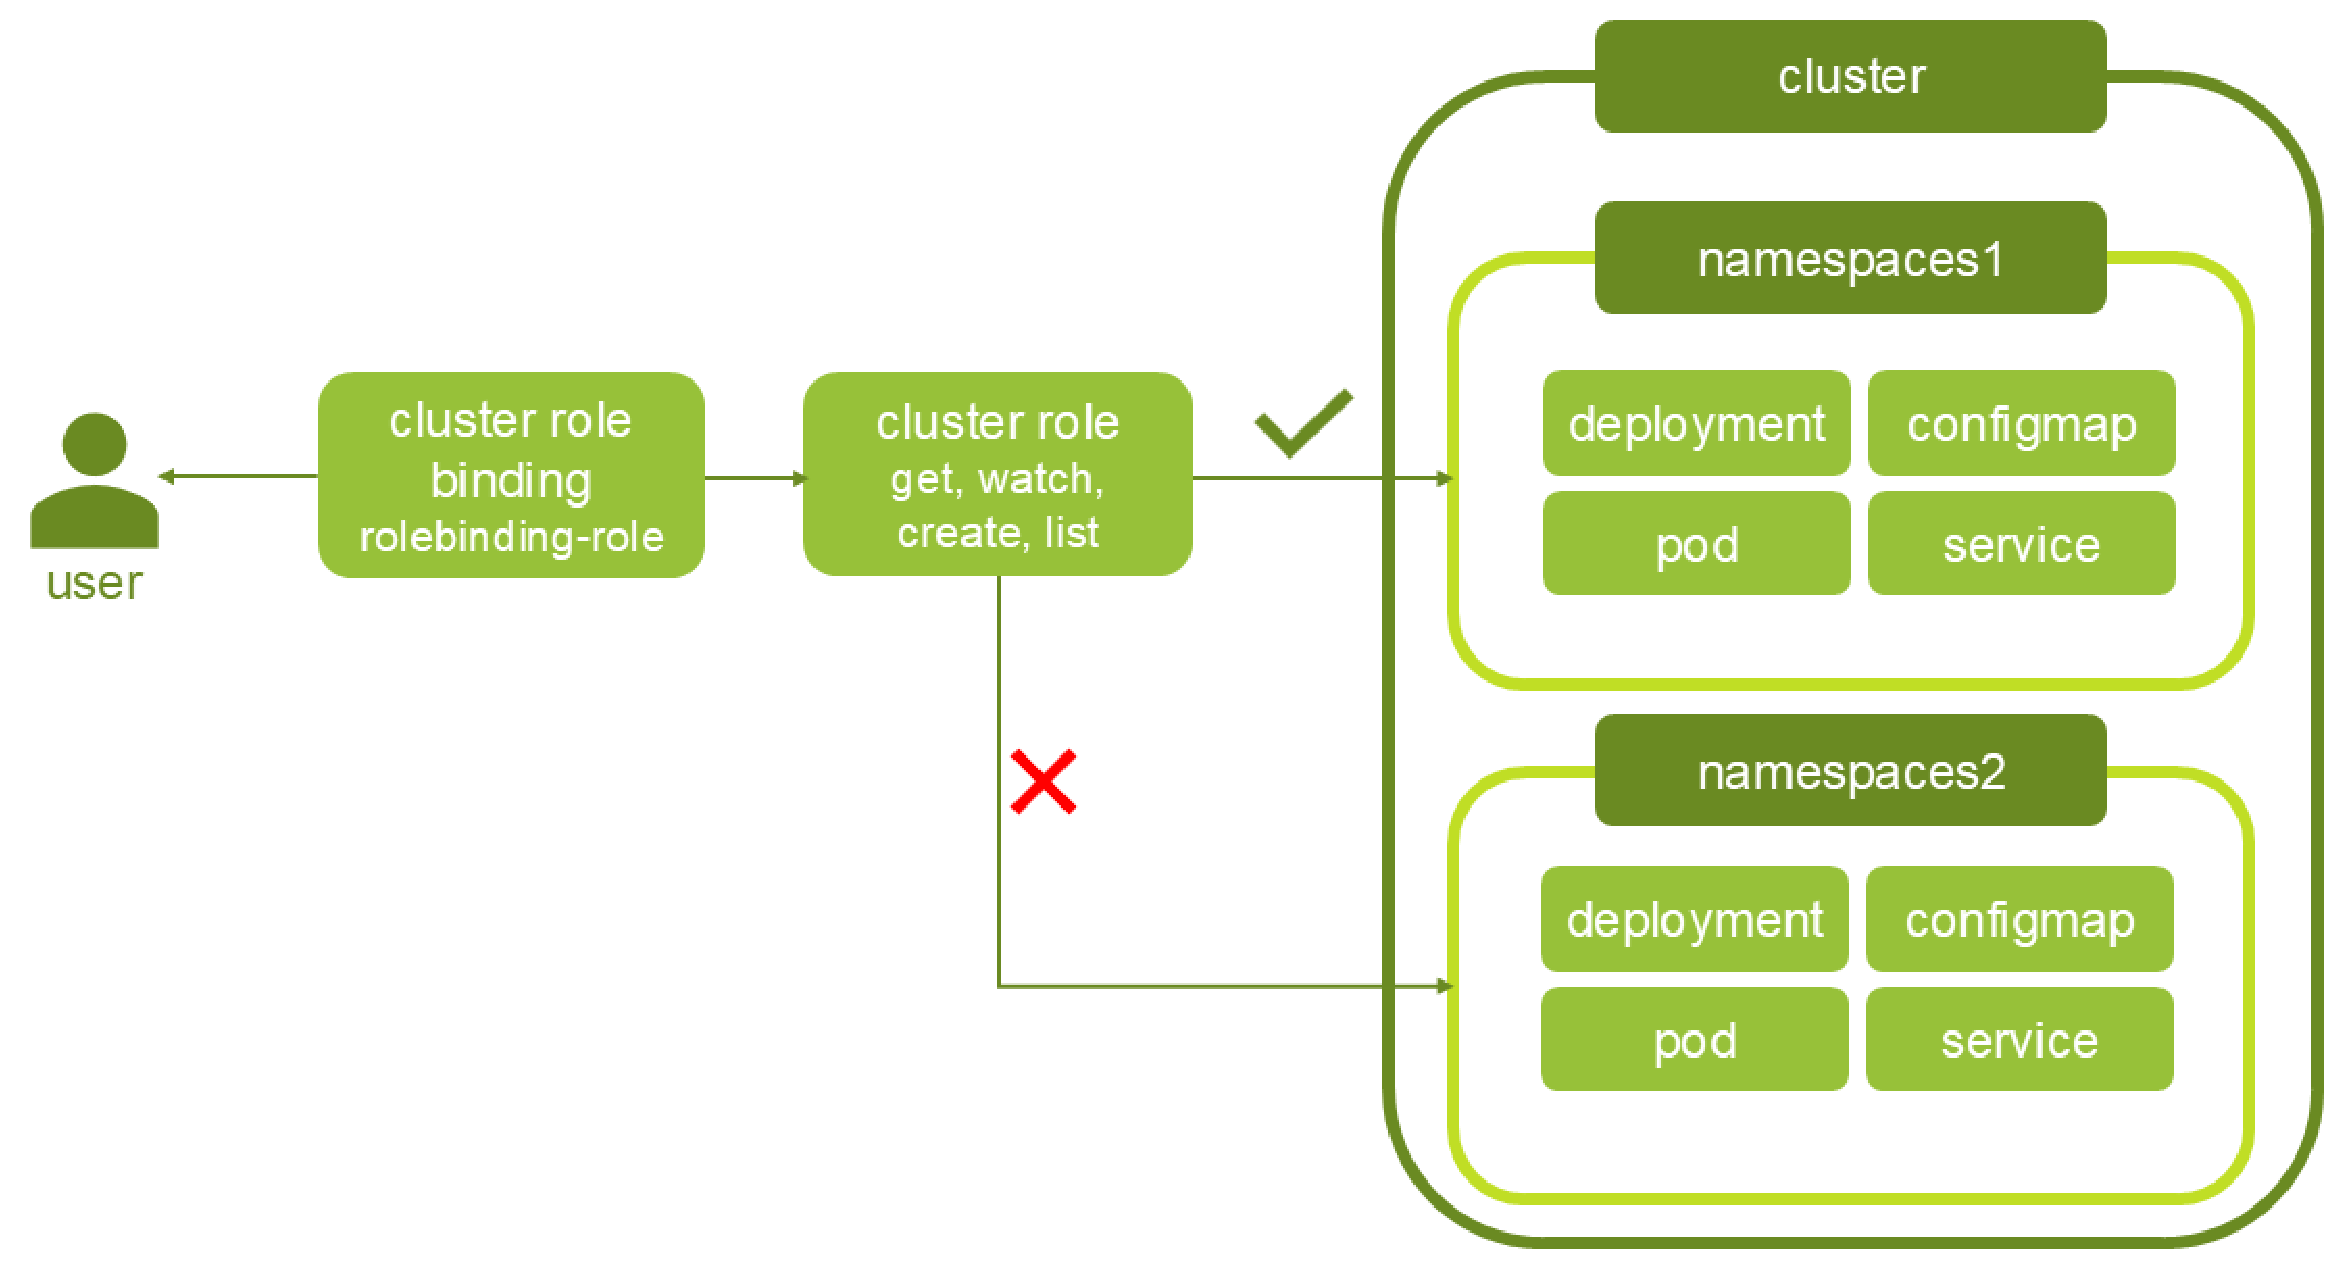
\includegraphics[width=1 \linewidth]{Thesis/Figures/Slide41.pdf}
\caption{\label{fig:RoleBinding}RoleBinding \cite{rahasak_Kubernetes_rbac}}
\end{figure}

\clearpage

\textbf{ClusterRoleBinding}

A ClusterRoleBinding, on the other hand, grants permissions cluster wide by associating a ClusterRole with one or more users, groups, or service accounts across the entire Kubernetes cluster. Unlike RoleBindings, which are confined to a single namespace, ClusterRoleBindings apply the permissions defined in a ClusterRole to all namespaces or to cluster scoped resources, as illustrated in the \autoref{fig:ClusterRoleBinding}. This makes ClusterRoleBindings ideal for granting broad access, such as allowing a group of managers to read secrets across all namespaces. Once a ClusterRoleBinding is created, it cannot be modified to reference a different role, if a change is needed, the binding must be deleted and recreated to ensure that the new roles permissions are intentionally granted to the subjects. \cite{Kubernetes_doc}


\captionsetup{justification=centering}
\begin{figure}[h]
\centering
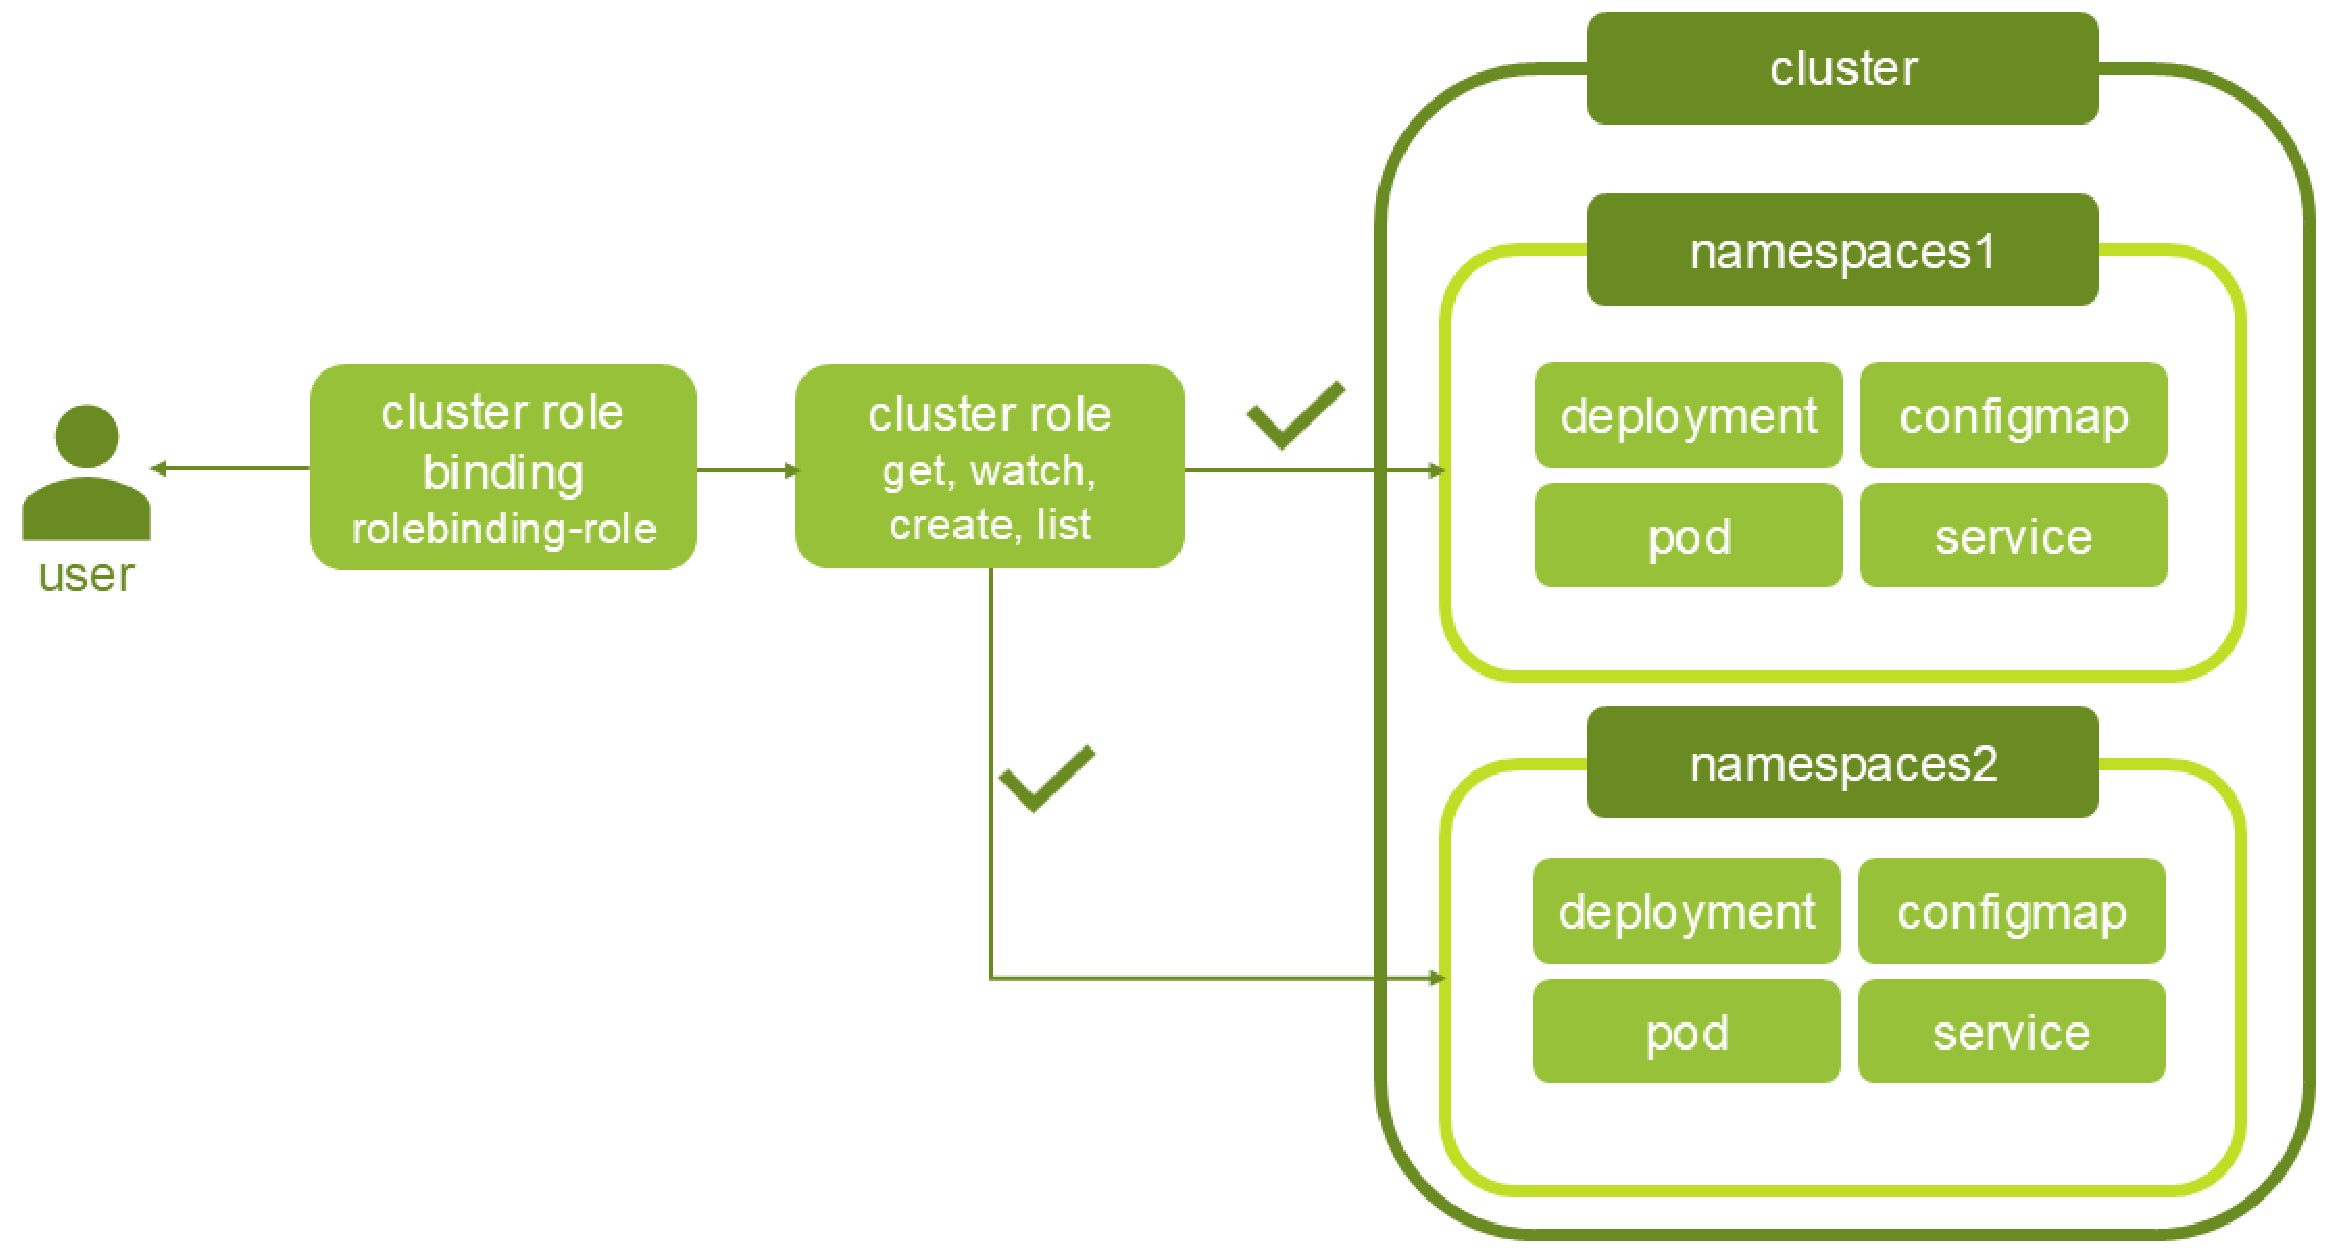
\includegraphics[width=1 \linewidth]{Thesis/Figures/Slide42.pdf}
\caption{\label{fig:ClusterRoleBinding}ClusterRoleBinding \cite{rahasak_Kubernetes_rbac}}
\end{figure}

\section{Scalable and Distributed Architecture for AI Models}

This section describes scalable and distributed architectures for AI models, focusing on concepts such as distributed and parallel computing, batch processing and frameworks that support large-scale workloads. It explains core architectural components, cluster management and autoscaling techniques to enable efficient model training and deployment.

\subsection{Distributed Computing}

Distributed computing is a system where multiple independent entities, often called nodes, collaborate to solve problems or tasks by sharing resources and information. These nodes operate in different physical or virtual locations, each potentially having its own hardware, software and tasks. Despite their independence, these nodes must coordinate their actions to achieve a common goal. This coordination involves managing communication between nodes, ensuring the system remains functional even if some nodes fail and optimizing the distribution of tasks to improve efficiency and performance as shown in \autoref{fig:Distributed Computing}. A defining characteristic of distributed computing is the diversity in how these systems are structured and operate. Nodes may work synchronously or asynchronously, communicate through message passing or shared memory. The challenges in distributed computing include managing communication costs, ensuring fault tolerance, coordinating tasks effectively and addressing uncertainty due to the lack of global knowledge among nodes. As a result, distributed computing is a complex and dynamic field, encompassing a wide range of models and techniques to address the varying needs and constraints of different applications. \cite{podc_roger_2015}

\captionsetup{justification=centering}
\begin{figure}[h]
\centering
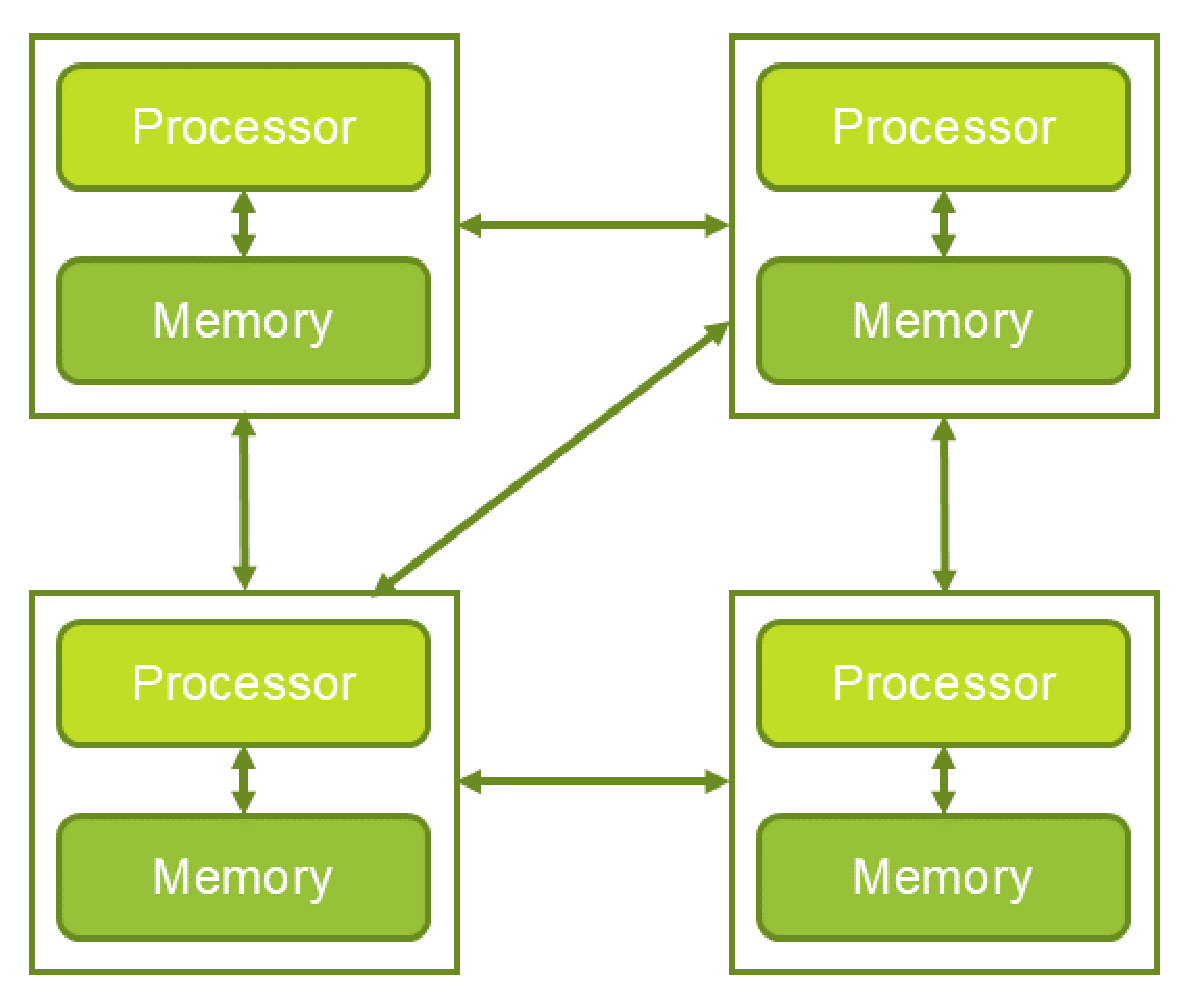
\includegraphics[width=0.7 \linewidth]{Thesis/Figures/Slide43.pdf}
\caption{\label{fig:Distributed Computing}Distributed Computing \cite{parallel_vs_distributed}}
\end{figure}

\subsection{Parallel Computing}

Parallel processing involves performing multiple tasks at the same time by using multiple processors, known as CPUs. This method is essential for handling complex problems that exceed the capabilities of traditional sequential computing systems. By dividing a task into smaller sub tasks through techniques such as divide and conquer and assigning these sub tasks to different processors, parallel processing significantly enhances computational efficiency and performance. This approach allows for the concurrent handling of diverse processes, which leads to a substantial increase in computing power compared to single processor systems as shown in \autoref{fig:Parallel Computing}. The push towards parallel processing is driven by several factors, including the growing computational demands of scientific and business applications. Sequential processors are reaching their performance limits due to physical constraints and the diminishing returns of hardware improvements like pipelining architectures. While vector processing works well for certain scientific applications, it is less effective for more general use cases. However, advances in parallel processing technology and networking have made it a viable and commercially exploitable solution, facilitating the development of more powerful and versatile computing systems. \cite{buyya2012microkernel}

\captionsetup{justification=centering}
\begin{figure}[h]
\centering
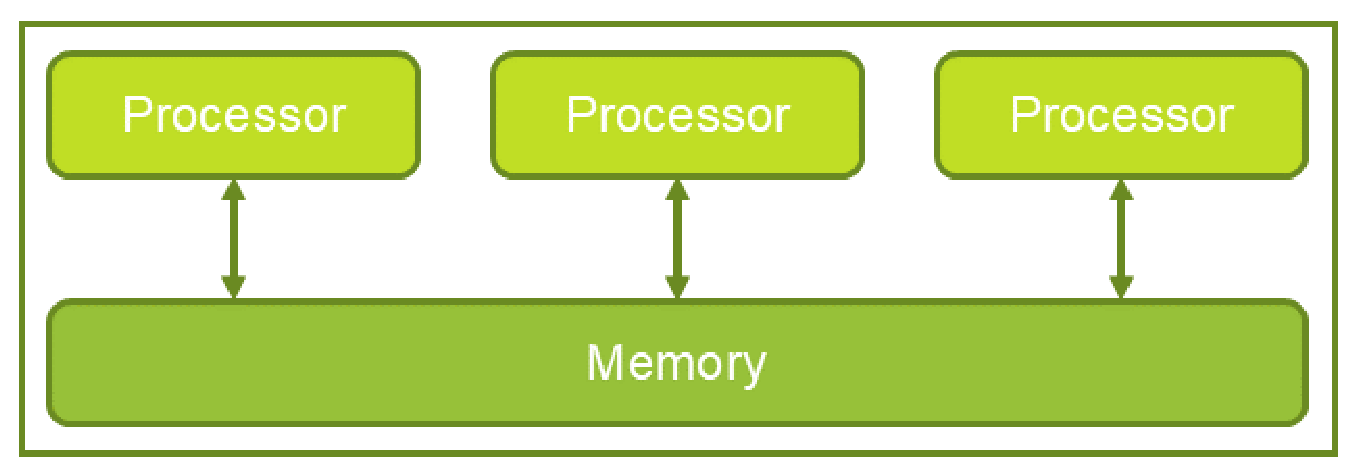
\includegraphics[width=0.9 \linewidth]{Thesis/Figures/Slide44.pdf}
\caption{\label{fig:Parallel Computing}Parallel Computing \cite{parallel_vs_distributed}}
\end{figure}



\subsection{Batch Processing}
Batch processing is a computing technique where a set of tasks or jobs is processed in a group or batch rather than individually as shown in \autoref{fig:Batch Processing}. This method is particularly efficient for handling large volumes of data or executing repetitive tasks with minimal human intervention. By queuing jobs and processing them sequentially, batch processing can optimize resource utilization and improve overall system throughput. For instance, in large-scale data analysis, batch processing allows for the aggregation and analysis of massive datasets in a structured and efficient manner, reducing the overhead associated with constant task switching and manual processing. The primary advantages of batch processing include its ability to perform operations during off peak hours, which minimizes the impact on system performance during peak times. Additionally, it supports automation and scheduling, which can significantly enhance productivity and reduce human error \cite{silberschatz2011database}. However, batch processing can introduce latency because jobs are only processed at scheduled intervals, which may not be suitable for applications that require real-time data processing. As a result, balancing batch processing with real-time systems is critical to optimising performance in different computing environments. \cite{tanenbaum2009modern}

\captionsetup{justification=centering}
\begin{figure}[h]
\centering
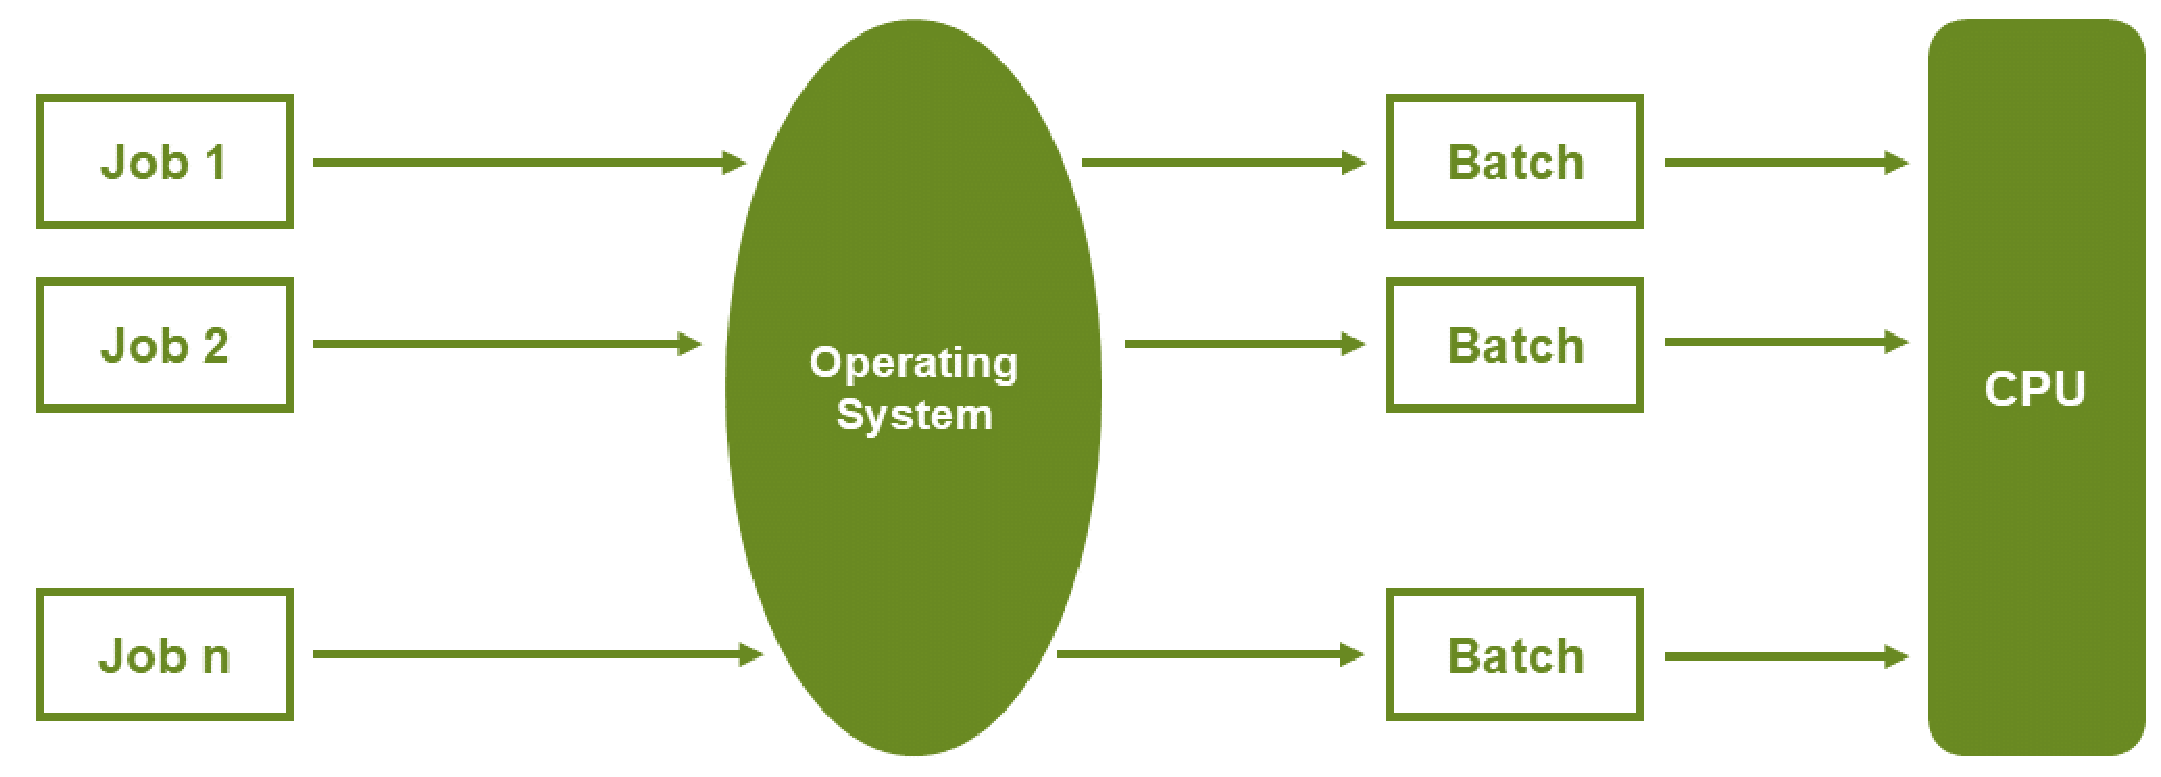
\includegraphics[width=0.9 \linewidth]{Thesis/Figures/Slide45.pdf}
\caption{\label{fig:Batch Processing}Batch Processing \cite{batch_processing_os}}
\end{figure}

\subsection{Ray Framework}

Ray is an open source framework that makes it easy to scale AI and ML applications with minimal effort. It enables developers to efficiently build distributed applications using a simple, flexible API. Ray core features include parallel and distributed computation, enabling the scaling of machine learning models across multiple nodes with minimal code changes. It supports a range of libraries based on Ray core, such as Ray data for distributed data processing, Ray train for ML and DL model training, Ray tune for hyperparameter tuning as shown in \autoref{fig:Ray Framework}. These features make Ray particularly advantageous for AI model deployment and scaling, as it abstracts the complexity of distributed computing, allowing researchers and engineers to focus more on model development rather than the underlying infrastructure. \cite{anyscale_blog}

The primary advantages of using Ray for AI model deployment include its ease of use, flexibility and robust performance. Ray architecture supports both stateless and stateful computations, enabling it to handle a wide variety of workloads. Additionally, Ray offers fault tolerance and dynamic resource management, which are critical for maintaining performance and reliability in large-scale AI systems. These capabilities are particularly beneficial for scaling AI models, as they allow for seamless integration and execution across diverse computational environments, from single machines to large clusters. Ray's flexibility and efficiency make it an optimal selection for the development and deployment of scalable AI applications. \cite{ray_doc}


\captionsetup{justification=centering}
\begin{figure}[h]
\centering
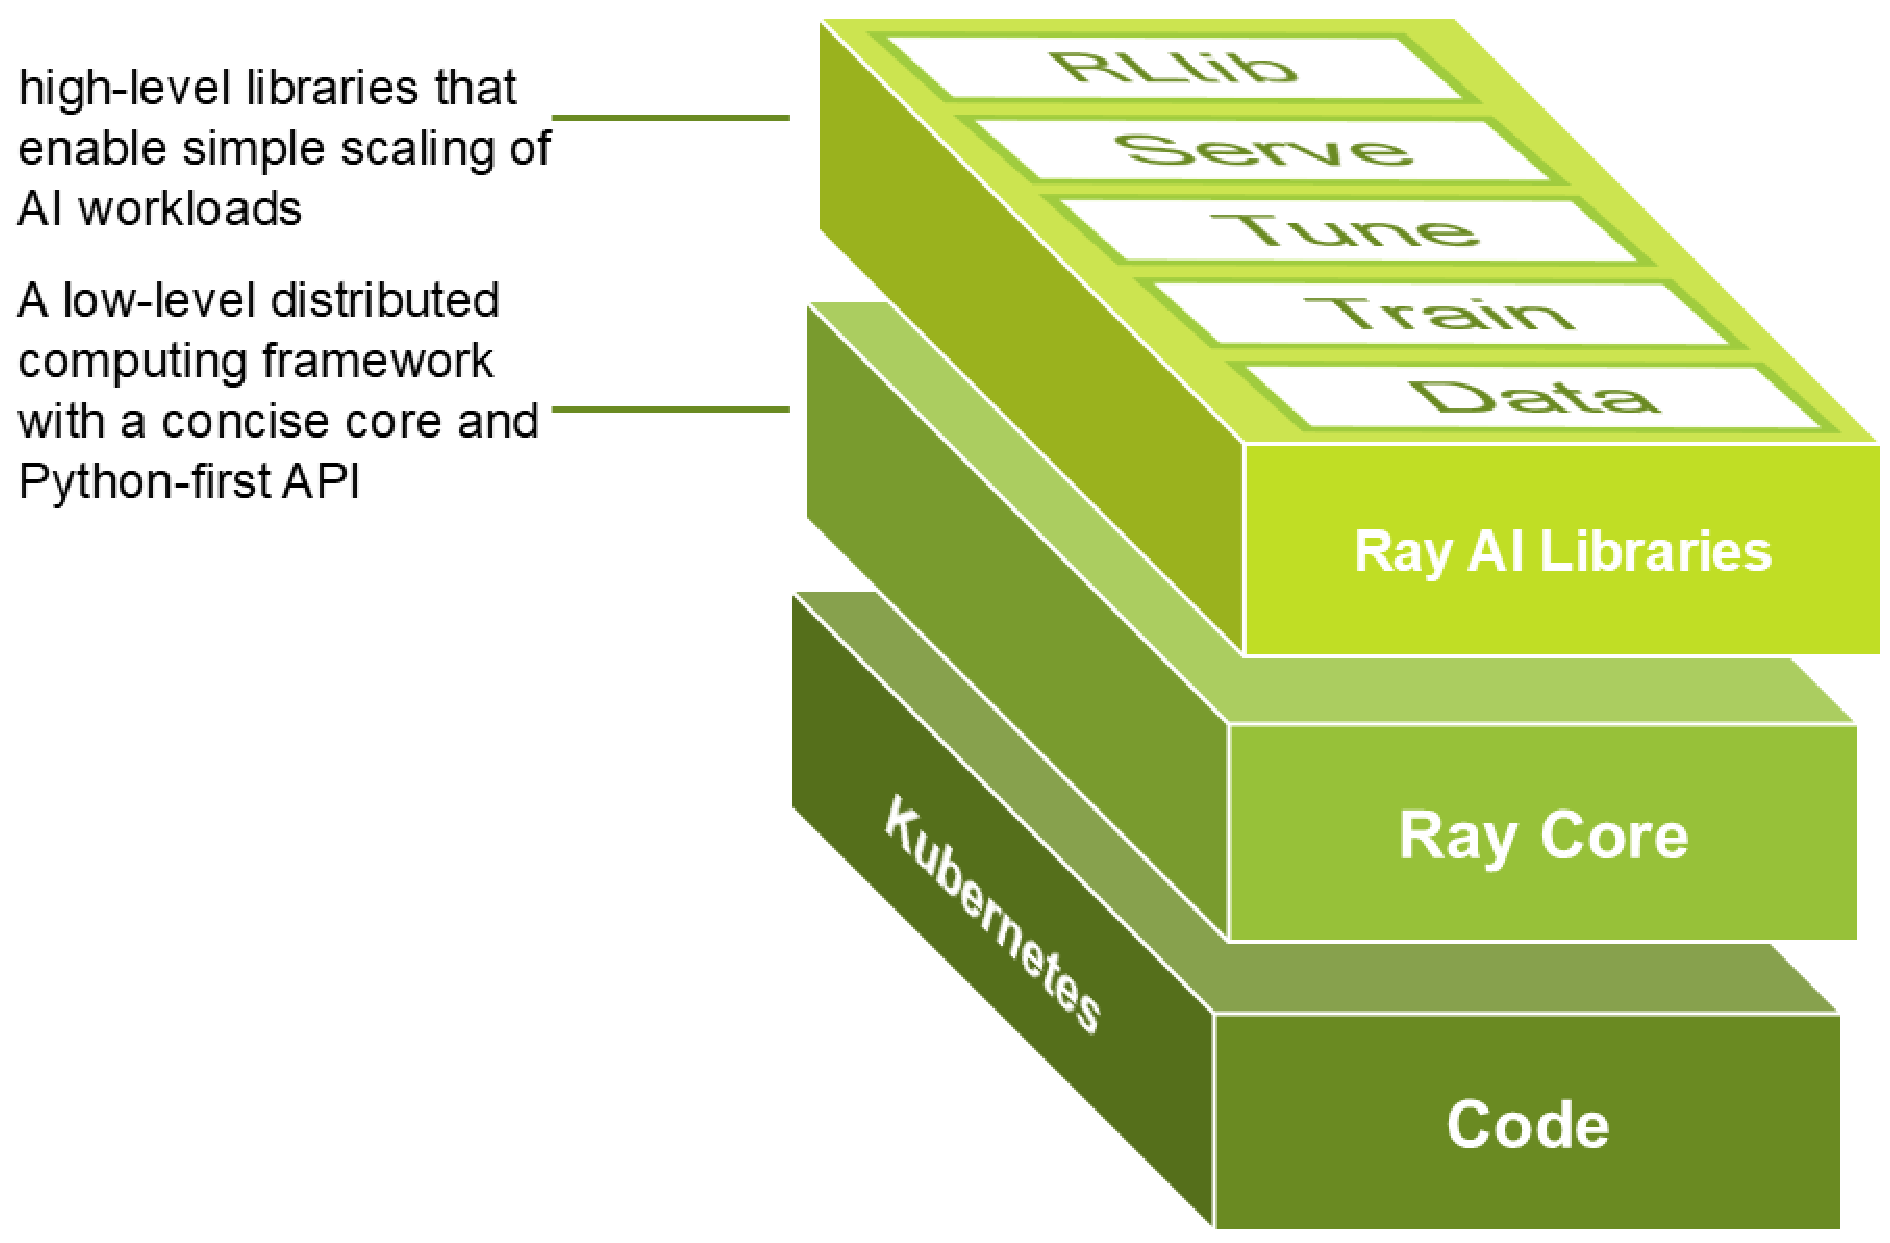
\includegraphics[width=1 \linewidth]{Thesis/Figures/Slide31.pdf}
\caption{\label{fig:Ray Framework}Ray Framework \cite{ray_doc}}
\end{figure}


\subsection{Ray Architecture}

Ray architecture is consist of two types of nodes, the head nodes and the worker nodes. A Ray head node is defined as a compute instance that executes the Ray components. Where a worker node is responsible for executing tasks based on Python process that is embedded within the head node. The head node is responsible for managing metadata and can be accessed by other nodes within the cluster. The head node contains a global control store, which provides assistance to workers in locating large objects within the cluster. The head node is furnished with a Raylet, comprising a scheduler for the administration of resources and an object store for the management of memory and state. The structure of the worker node is analogous to that of the head node, although it lacks the global control store and driver process. Each worker node is furnished with its own Raylet, which is responsible for the supervision of resource management and the administration of the object store as shown in \autoref{fig:Ray Architecture}. The distributed object store enables the sharing of large objects among worker nodes. The location of these objects can be determined by utilising the metadata stored within the global control store. Ray facilitates dynamic scaling, allowing for the addition or removal of worker nodes during the execution of an application. \cite{r34}



\captionsetup{justification=centering}
\begin{figure}[h]
\centering
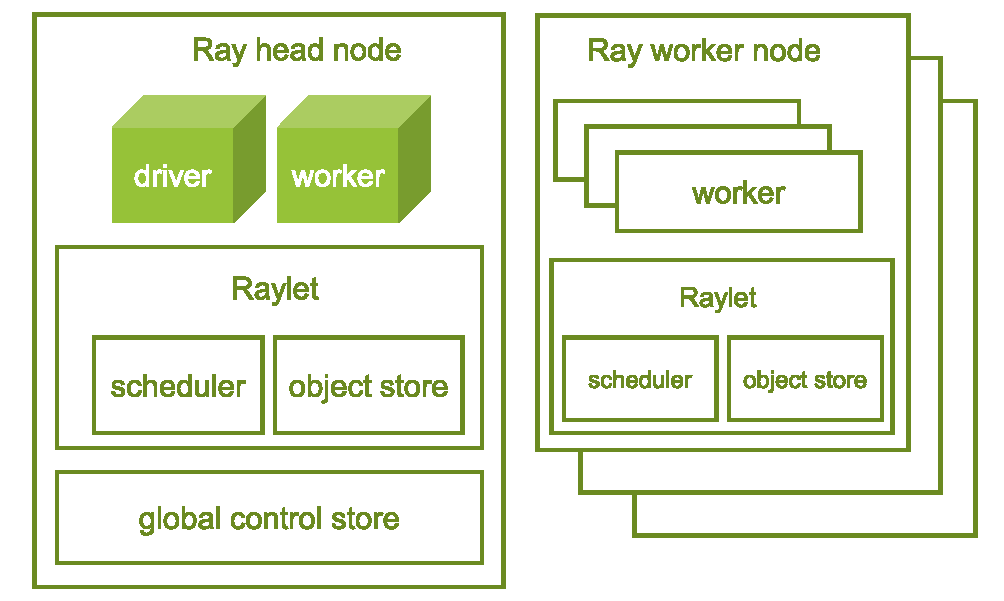
\includegraphics[width=1 \linewidth]{Thesis/Figures/Slide15.pdf}
\caption{\label{fig:Ray Architecture}Ray Architecture \cite{r34}}
\end{figure}


\subsection{Ray Cluster}

Ray enables seamless scaling of workloads from a single laptop to a large cluster. To run Ray applications across multiple nodes, deploying a Ray cluster is necessary. A Ray cluster comprises a head node and multiple worker nodes, which can be configured to autoscale based on the resource demands of the applications. This flexibility allows Ray clusters to efficiently handle varying workloads by scaling up or down as required and shown in \autoref{fig:Ray Cluster}.
A Ray cluster with two worker nodes. Each node runs Ray helper processes to facilitate distributed scheduling and memory management. The head node runs additional control processes. \cite{ray_doc}


\captionsetup{justification=centering}
\begin{figure}[h]
\centering
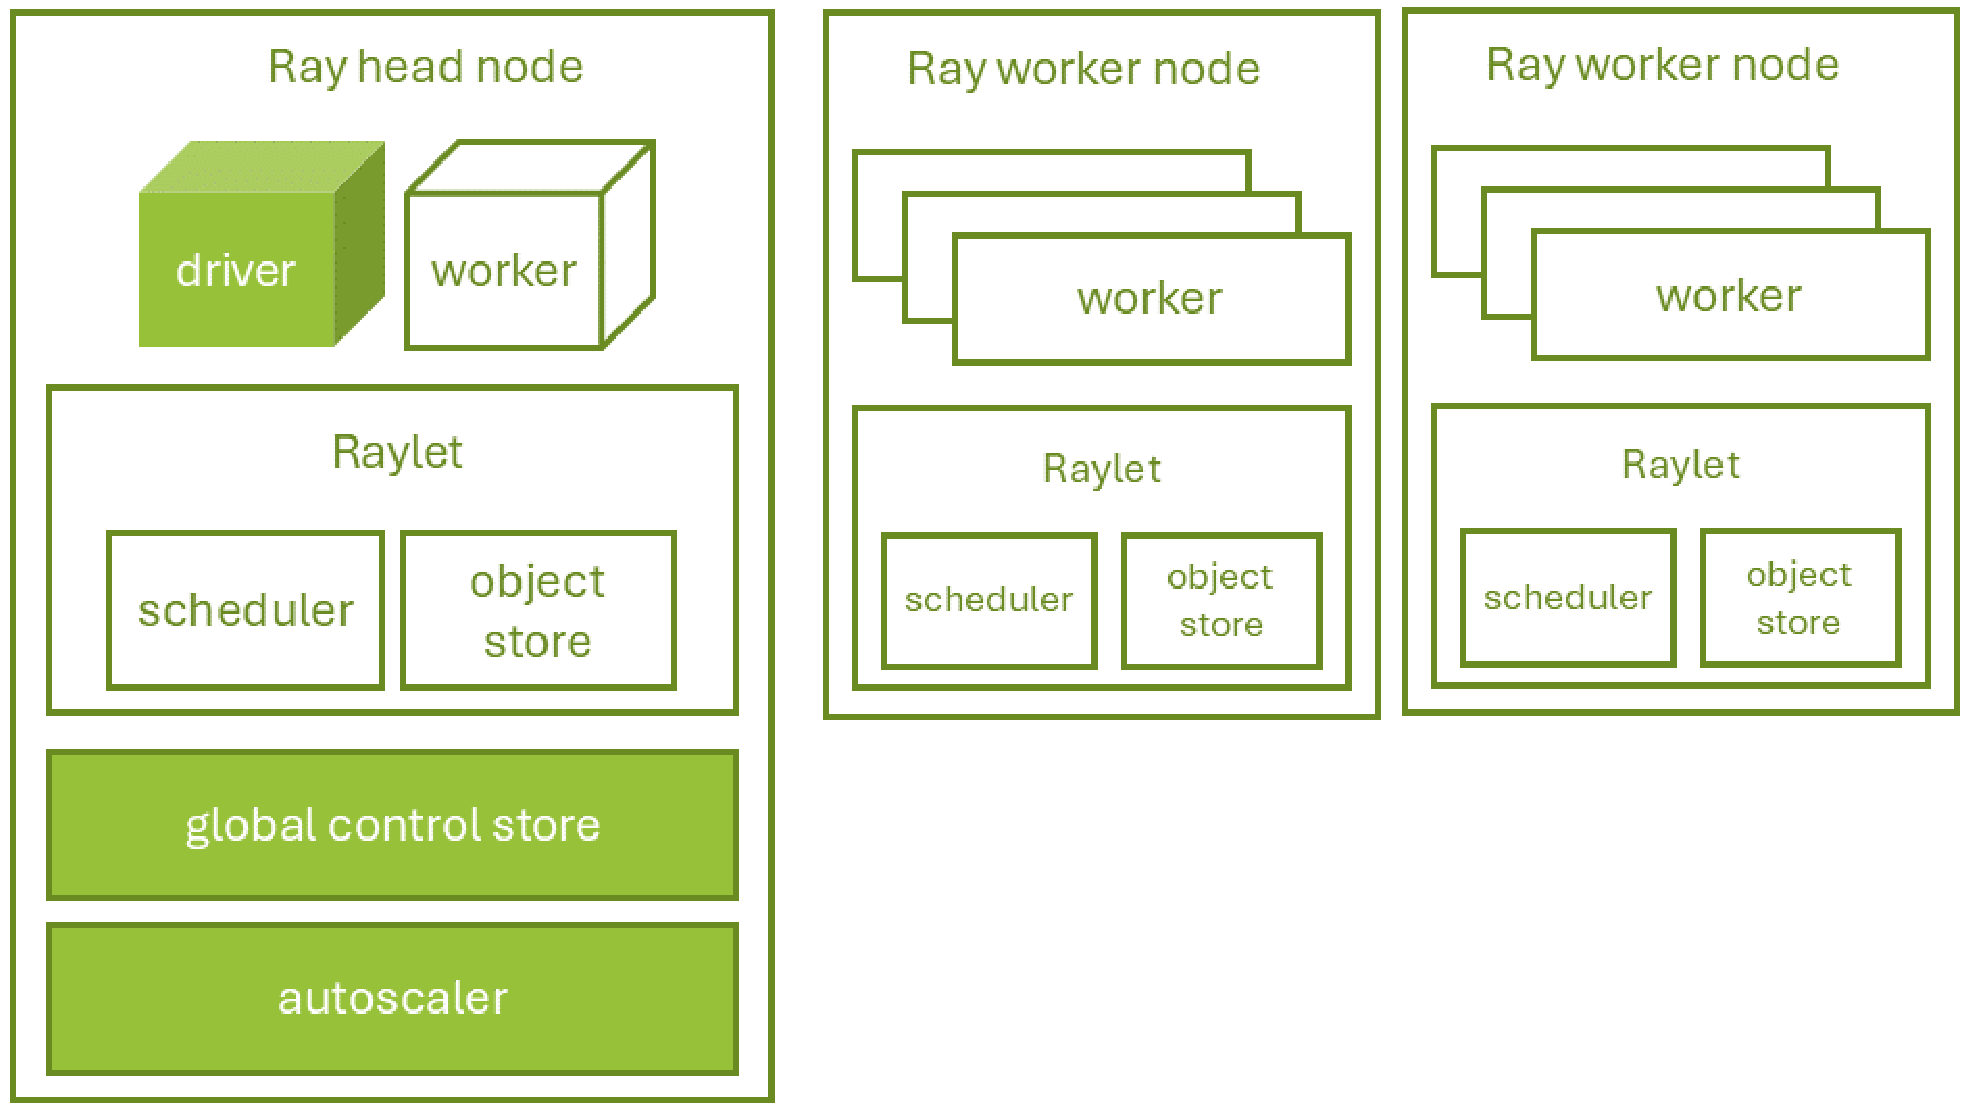
\includegraphics[width=1 \linewidth]{Thesis/Figures/Slide40.pdf}
\caption{\label{fig:Ray Cluster}Ray Cluster Architecture \cite{ray_doc}}
\end{figure}

\textbf{Head Node}

Each Ray cluster has a designated head node, which differs from worker nodes in that it manages cluster operations. The head node runs several essential singleton processes including the autoscaler, the global control store and the Ray driver processes responsible for executing Ray jobs. Although the head node can participate in task scheduling and actor management like any other worker node, it is generally recommended to avoid running tasks on it in large-scale clusters. This ensures optimal performance and resource allocation across the cluster. \cite{ray_doc}

\textbf{Worker Node}

Worker nodes are integral to running user code within Ray tasks and actors. Unlike the head node, worker nodes do not handle cluster management processes. Instead, they focus on distributed scheduling, storage and distribution of Ray objects within the cluster memory. The primary role of worker nodes is to execute tasks and actors, thus enabling efficient parallel processing across the cluster. \cite{ray_doc}

\textbf{Autoscaling}

The autoscaler, a process that operates on the head node or as a sidecar container in Kubernetes environments, manages the dynamic adjustment of worker nodes. When the resource demands of the Ray workload surpass the cluster’s current capacity, the autoscaler increases the number of worker nodes. Conversely, it will reduce the number of worker nodes when there is idle capacity. It is crucial to note that the autoscaler responds to task and actor resource requests rather than application metrics or physical resource utilization. \cite{ray_doc}

\clearpage

\textbf{Ray Jobs}

A Ray job refers to a single application consisting of Ray tasks, objects and actors derived from the same script. The worker running the Python script is termed the driver of the job. Ray jobs can be executed in two main ways as shown in \autoref{fig:Ray Job} by submitting the job using the Ray jobs API, which is the recommended approach, or by running the driver script directly on the Ray cluster for interactive development. The Ray jobs API guide provides additional details on these workflows. \cite{ray_doc}


\captionsetup{justification=centering}
\begin{figure}[h]
\centering
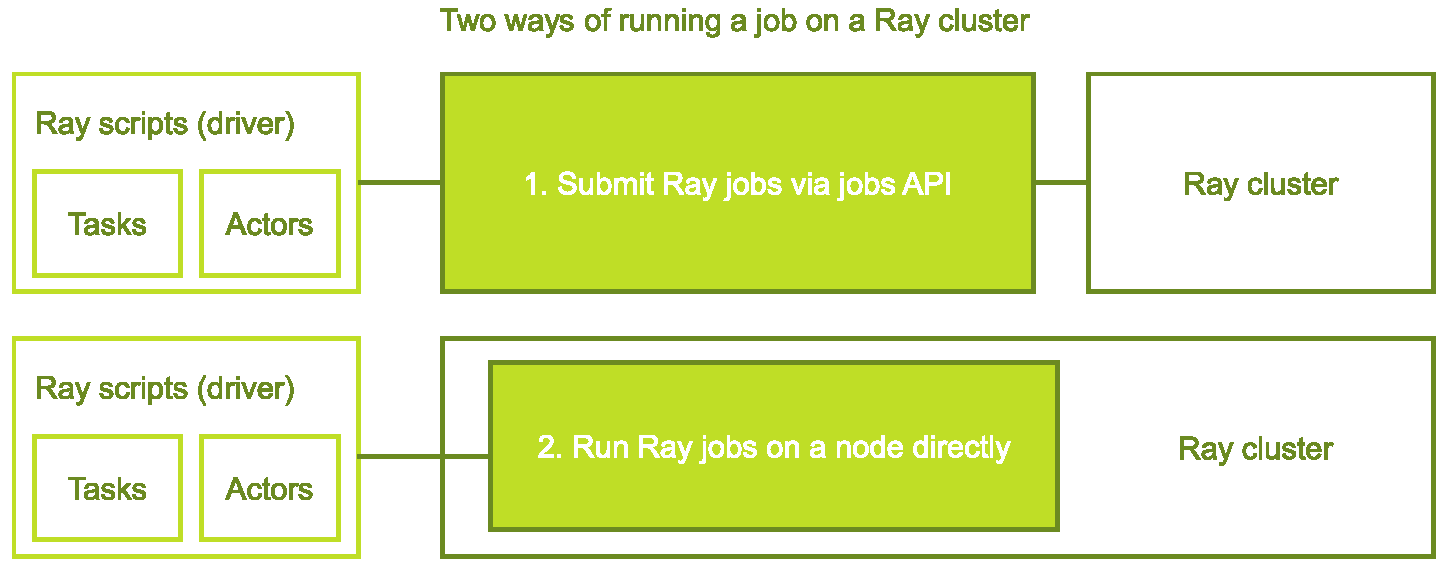
\includegraphics[width=1 \linewidth]{Thesis/Figures/Slide22.pdf}
\caption{\label{fig:Ray Job}Ray Job \cite{ray_doc}}
\end{figure}



\subsection{KubeRay Operator}

The KubeRay operator is a Kubernetes native operator designed to manage Ray clusters on Kubernetes efficiently. It simplifies the deployment, scaling and management of Ray clusters by leveraging Kubernetes robust orchestration capabilities. By using the KubeRay operator, developers can benefit from Kubernetes features such as automated rollouts, rollbacks, service discovery and resource management, which are seamlessly integrated into Ray architecture. This integration allows for enhanced scalability and reliability of distributed AI workloads running on Ray. The KubeRay operator defines custom resource definitions \abk{CRD}{Custom Resource Definitions} that represent the desired state of a Ray cluster. It ensuring that the cluster remains in optimal condition by continuously monitors the actual state of the cluster and reconciles it with the desired state. This includes managing Ray head and worker nodes shown in \autoref{fig:KubeRay Operator}, handling node failures and scaling the cluster based on workload demands. By automating these tasks the KubeRay operator reduces the operational burden on developers and enables them to focus more on developing AI models and less on infrastructure management.This integration of Ray with Kubernetes through the KubeRay operator provides a powerful solution for delivering and managing scalable AI applications in a cloud-native architecture. \cite{anyscale_blog, ray_doc}

\clearpage

\captionsetup{justification=centering}
\begin{figure}[h]
\centering
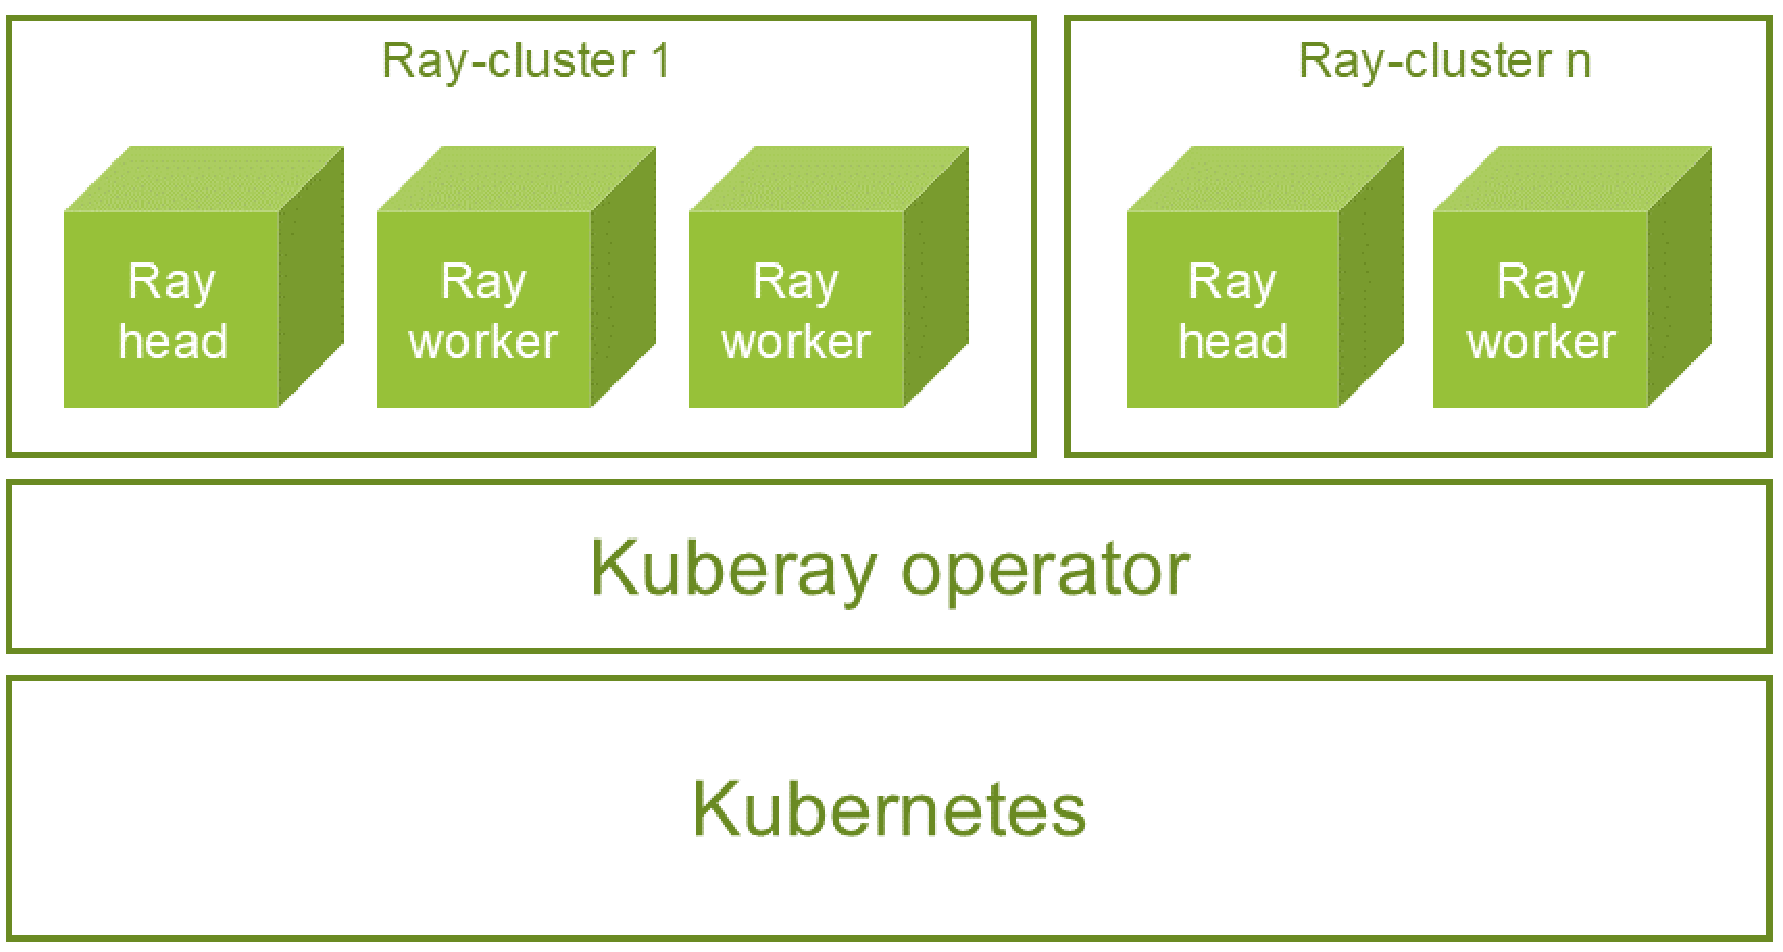
\includegraphics[width=1 \linewidth]{Thesis/Figures/Slide14.pdf}
\caption{\label{fig:KubeRay Operator}KubeRay Operator \cite{r34}}
\end{figure}

\subsection{Ray Core}

Ray core is the fundamental building block of the Ray ecosystem, it offers a distributed execution engine that support scalability and parallelism required for AI and ML workloads. The setup Ray core environment Helm charts or Kubernetes manifests is used, which outline the required configuration for Ray components. Configurations typically specify the cluster size, resource allocations and environment variables, ensuring that the Ray cluster can dynamically scale in response to workload demands. Ray core serves as the backbone for other Ray libraries, such as Ray tune, Ray train and Ray serve. It manages distributed task scheduling, state management and fault tolerance which are essential for the efficient execution of parallel computations. The integration of Ray core with Kubernetes through KubeRay allows for advanced features like autoscaling and resource management, ensuring that the cluster adapts to varying workloads while maintaining optimal performance. \cite{ray_doc}


\textbf{Ray Task}

Ray tasks are functions that can be executed remotely, allowing them to run concurrently across different nodes in the cluster. These tasks are defined using the \texttt{@Ray.remote} decorator and their execution is managed by distributed scheduler of Ray. The code snippet \autoref{listingsnippet:3} shows, a simple Ray task. This task will be executed on one of the available worker nodes and the result will be returned to the head node. \cite{ray_doc}


\listingsnippet{Ray Task Example \cite{ray_doc}}{

\vspace{0.3cm}

\hspace{0.25cm}\texttt{import ray}

%\vspace{0.1cm}

\hspace{0.25cm}\texttt{ray.init()}

%\vspace{0.1cm}

\hspace{0.25cm}\texttt{@ray.remote}

\vspace{0.3cm}

\hspace{0.25cm}\texttt{def mytask(x):}

\hspace{0.75cm}\texttt{return x + x}

\vspace{0.3cm}

\hspace{0.25cm}\texttt{result = ray.get(my-task.remote(4))}


\hspace{0.25cm}\texttt{print(result)  \# Output: 8}

\vspace{0.3cm}
}


\textbf{Ray Actor}

Ray actors extend the concept of Ray task by allowing stateful computations. An actor is essentially a Python class where each method invocation is treated as a remote task. Actors are particularly useful when managing state across tasks, as they maintain their state in-memory across multiple invocations. Code snippet \autoref{listingsnippet:4} shows the example how actors are used in scenarios where maintaining state consistency across distributed tasks is critical. \cite{ray_doc}

\listingsnippet{Ray Actor Example \cite{ray_doc}}{

\vspace{0.3cm}

\hspace{0.25cm}\texttt{@ray.remote}

\hspace{0.25cm}\texttt{class Counter:}

\vspace{0.3cm}

\hspace{0.75cm}\texttt{def init(self):}

\hspace{1.5cm}\texttt{self.count = 0}

\vspace{0.3cm}

\hspace{0.75cm}\texttt{def increment(self):}

\hspace{1.5cm}\texttt{self.count += 1}

\hspace{1.5cm}\texttt{return self.count}

\vspace{0.3cm}

\hspace{0.25cm}\texttt{counter = Counter.remote()}

\hspace{0.25cm}\texttt{print(ray.get(counter.increment.remote()))  \# Output: 1}

}


\textbf{Ray Core Methods}

Ray Core provides a number of methods that facilitate distributed computing. These methods simplify the process of parallelizing and distributing tasks across a cluster of machines. Key methods include

\begin{itemize}
    \item Ray.init()
    \item Ray.remote()
    \item Ray.get()
    \item Ray.put()
    \item Ray.shutdown()
\end{itemize}

The \texttt{Ray.init()} method initializes the Ray runtime and connects the Python program to the Ray cluster. It's the first step in setting up a Ray program and can be configured to connect to either a local Ray instance or a remote cluster. The \texttt{Ray.remote()} decorator is used to define Ray tasks or actors. By marking a Python function or class with \texttt{Ray.remote}, It automatically distributes the function execution or class instantiation across the cluster, allowing parallel computation. The \texttt{Ray.get()} method is used to retrieve results from Ray tasks or actor methods. As Ray executes tasks asynchronously, \texttt{Ray.get()} is used to block execution until the results are available to facilitate synchronization across the distributed system. The \texttt{Ray.put()} method allows large objects to be stored in the distributed object store so that they can be shared efficiently between tasks and actors without duplication, thus optimising memory usage in the cluster. Finally, the \texttt{Ray.shutdown()} method neatly shuts down the Ray runtime, ensuring that all tasks are completed and resources are properly freed, which is critical to maintain cluster stability. Ray core methods enable seamless interaction with the distributed system, allowing developers to focus on their application logic without worrying about the complexities of distributed computing. These methods, combined with the orchestration capabilities of Kubernetes, provide a powerful platform for scaling AI and ML workloads. \cite{ray_doc}


\textbf{Sequential Implementation}

In a sequential implementation of Ray, tasks or functions are executed one at a time, in a single thread or process, as shown in \autoref{fig:sequential}. This traditional approach works well for simpler workloads or where the overhead of parallelism outweighs the benefits. However, it limits the ability to take full advantage of multi-core CPUs and distributed systems. In this mode, Ray behaves like a normal Python program, where each function is executed in the order it's called and the system waits for the current task to finish before moving on to the next. This limits scalability, but can be easier to debug and manage for small tasks. \cite{ray_doc}



\begin{figure}[h]
\centering
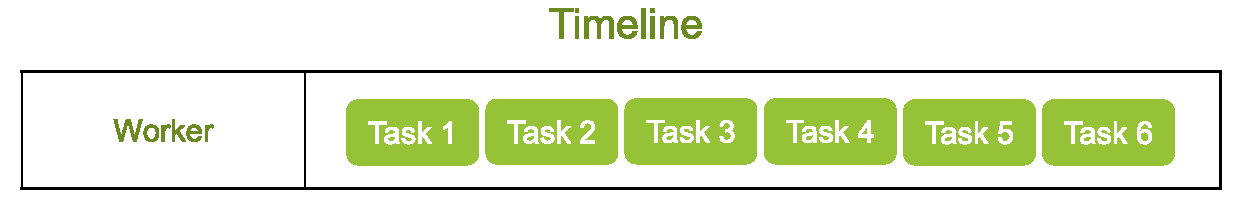
\includegraphics[width=1 \linewidth]{Thesis/Figures/Slide68.pdf}
\caption{\label{fig:sequential}Sequential Implementation of Tasks \cite{ray_doc}}
\end{figure}



\textbf{Parallel Implementation}

Parallel implementation of Ray, uses all available resources to train models in parallel, maximizing computational efficiency. Ray automatically detects the number of cores on your machine, or the available resources in a cluster and dynamically distributes each task across them as shown in \autoref{fig:parallel}. Instead of processing tasks sequentially, Ray introduces a scheduler that manages incoming requests, assigns them to nodes and monitors resource availability to ensure optimal use. This parallel execution model accelerates processing by using multiple cores or machines simultaneously, resulting in significant performance improvements, especially for resource intensive tasks such as ML model training. \cite{ray_doc}

\clearpage

\begin{figure}[h]
\centering
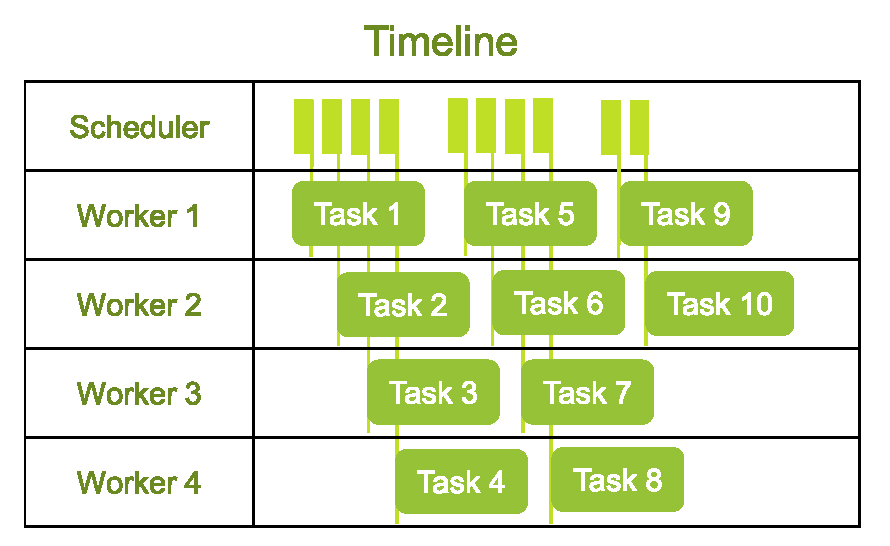
\includegraphics[width=1 \linewidth]{Thesis/Figures/Slide69.pdf}
\caption{\label{fig:parallel}Parallel Implementation of Tasks \cite{ray_doc}}
\end{figure}

\subsection{Ray Data}

Ray data is a key component of the Ray ecosystem, designed to handle large-scale data processing tasks in a distributed manner across multiple nodes within a cluster. It facilitates the seamless distribution of datasets, enabling parallel processing and transformation of data, which is essential for scaling ML and data intensive applications. By integrating with other Ray modules, Ray Data enables efficient handling of diverse workloads such as data loading, pre processing and transformation, while ensuring that operations are distributed to maximize resource utilization and minimize processing time. Ray Data emerges as the most suitable solution for scalable and high performance data processing. Ray Data provide the distributed processing capabilities to efficiently manage the dataset across the Ray cluster. Instead of relying on traditional single node data handling, the dataset was distributed across multiple nodes, ensuring that data loading and processing tasks were executed concurrently. This approach allows to scale operation with less processing time by distributing tasks across the cluster and achieve high level of parallelism as shown in \autoref{fig:Ray Data}, which significantly improved the throughput and responsiveness of our system. This implementation demonstrated the effectiveness of Ray Data in managing large-scale data processing workflows within a distributed environment, aligning with the goals of scalability and efficiency. \cite{ray_doc}

\clearpage

\begin{figure}[h]
\centering
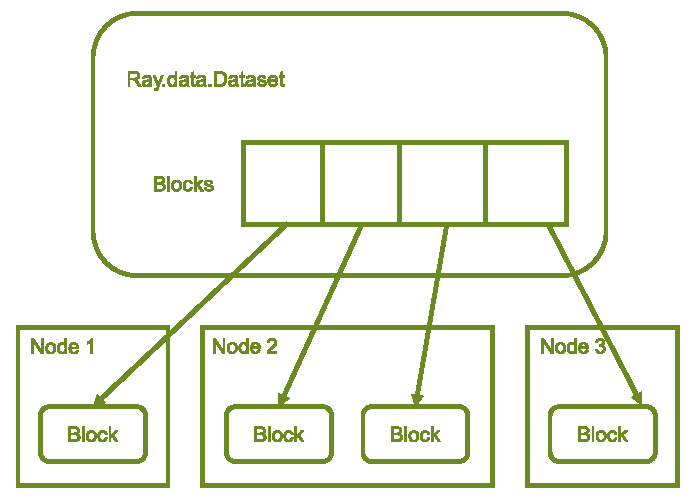
\includegraphics[width=0.9 \linewidth]{Thesis/Figures/Slide52.pdf}
\caption{\label{fig:Ray Data}Ray Data Overview \cite{anyscale_blog}}
\end{figure}



\subsection{Ray Train}

Ray train is a core component of the Ray ecosystem that enables distributed training of model across multiple nodes. It is designed to handle large ML and DL workloads by distributing tasks in parallel to speed up the training process. Ray train integrates easily with other ML frameworks and provides built-in fault tolerance ensuring continues training even if some nodes fail. This capability is particularly useful when working with large datasets that require high computational resources. By using Ray train ML engineers can optimise their training workflows, reducing required time and efficiently scaling operations within a Kubernetes environment. The training process in Ray is organized around several components, such as training function, worker, scaling configuration and trainer. The training function consist of the core logic of model training including loading dataset, defining model and performing training iterations. The function is distributed across multiple nodes by Ray train, allowing parallel processing. By assigning each worker a separate process to perform the training function. The workers are distributed across the cluster, allowing the training logic to be executed concurrently. The distribution of workers allows efficient use of computational resources, whether CPUs or GPUs. Scaling configurations specify the number of workers and the computing resources allocated to each worker. This configuration is critical for optimising resource usage and ensuring that the training workload is appropriately balanced across the cluster. The trainer class then brings together the training function, the workers and the scaling configuration and orchestrates the execution of the distributed training job, managing the distribution of data and synchronization of results across the workers. Ray train conduct large-scale distributed training effectively also shown in \autoref{fig:Ray Train}. The scalability and fault tolerance provided by Ray train were essential in managing complex training tasks within the Kubernetes environment, ensuring high performance and reliability. \cite{ray_doc}

\begin{figure}[h]
\centering
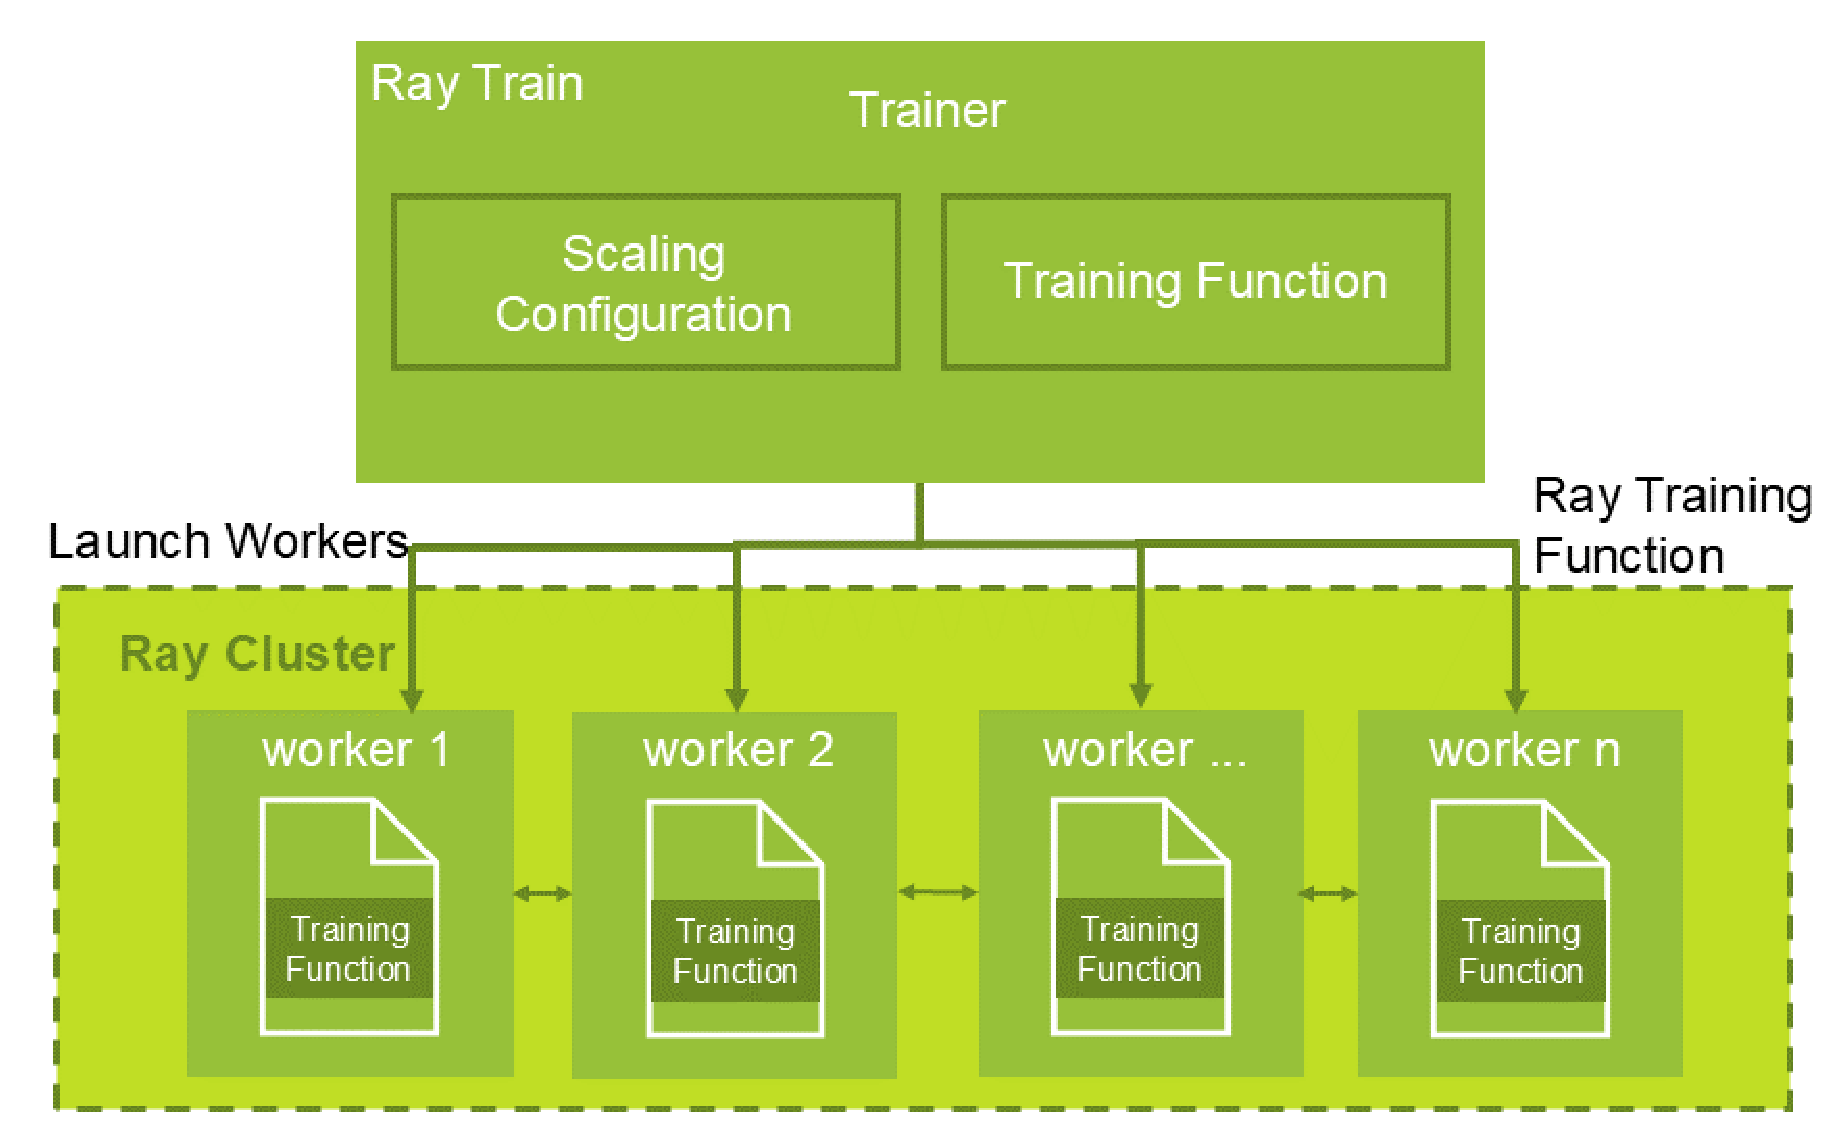
\includegraphics[width=1 \linewidth]{Thesis/Figures/Slide53.pdf}
\caption{\label{fig:Ray Train}Ray Train Overview \cite{ray_doc}}
\end{figure}


\subsection{Ray Tune}

Ray tune is a powerful optimization library that allows efficient exploration of hyperparameter spaces to find the best model configurations. It provides algorithms such as Population Based Training  and HyperBand to optimize and accelerate the tuning process.  Ray tune handles hyperparameter optimization by defining a search space for critical hyperparameters such as the number of estimators and the maximum depth of trees. Using this search space Ray tune can explore different combinations of these hyperparameters. Ray tune integration into the Ray ecosystem facilitates the distributed execution of hyperparameter optimization tasks. By utilizing the computational resources of Ray cluster, distributed tuning of workload across multiple nodes are possible see \autoref{fig:Ray Tune}, which significantly accelerated the optimization process. This distributed approach ensures that hyperparameter tuning is efficient and scalable, making it suitable for large-scale ML tasks. Ray tune also provides built-in support for logging and tracking the results of each trial. \cite{ray_doc}


\clearpage

\begin{figure}[h]
\centering
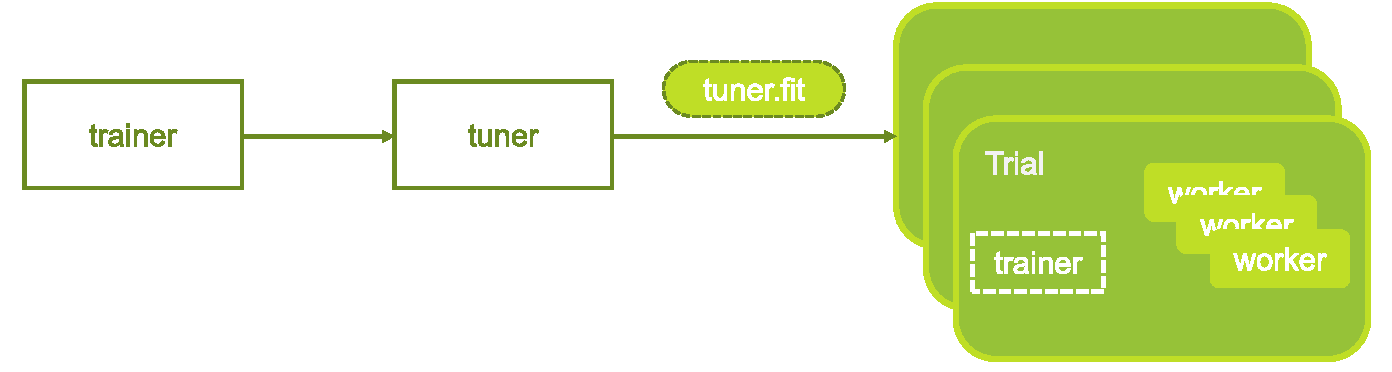
\includegraphics[width=1 \linewidth]{Thesis/Figures/Slide55.pdf}
\caption{\label{fig:Ray Tune}Ray Tune Overview \cite{ray_doc}}
\end{figure}



\subsection{Autoscaling with Ray}

Autoscaling of resources using Ray involves sequence of steps to achieve efficient resource utilization and performance of ML and DL workloads. First, Ray cluster must be configured to dynamically adjust the number of worker nodes based on the workload requirements. This is achieved through Ray autoscaler by defining the minimum and maximum number of nodes in a configuration file. Once autoscaler is configured, its start monitoring the resource usage and workload demands and automatically adds or remove worker nodes as needed to meet the workload demand. This dynamic scaling capability helps in optimizing resource allocation, reducing costs and maintaining high performance under varying workloads as shown in \autoref{fig:Autoscaling with Ray}. \cite{moritz}

Performance optimization techniques are crucial when enabling autoscaling with Ray. Key strategies of optimizing performance includes monitoring system metrics to identify bottlenecks, optimizing the configuration of worker nodes and fine tuning the scheduling policies to improve resource utilization. Additionally, leveraging Ray built-in libraries, such as tune for hyperparameter optimization and reinforcement learning libraries \abk{RLlib}{Reinforcement Learning Library}, can further enhance the efficiency and effectiveness of AI models. Developers can ensure that the system operates at peak, by continuously analyzing and adjusting the resource allocation, which provides a robust and scalable solution for deploying AI models in production environments. \cite{r52}

\makeatletter
\setlength{\@fptop}{0pt}
\makeatother


\begin{figure}[h]
\centering
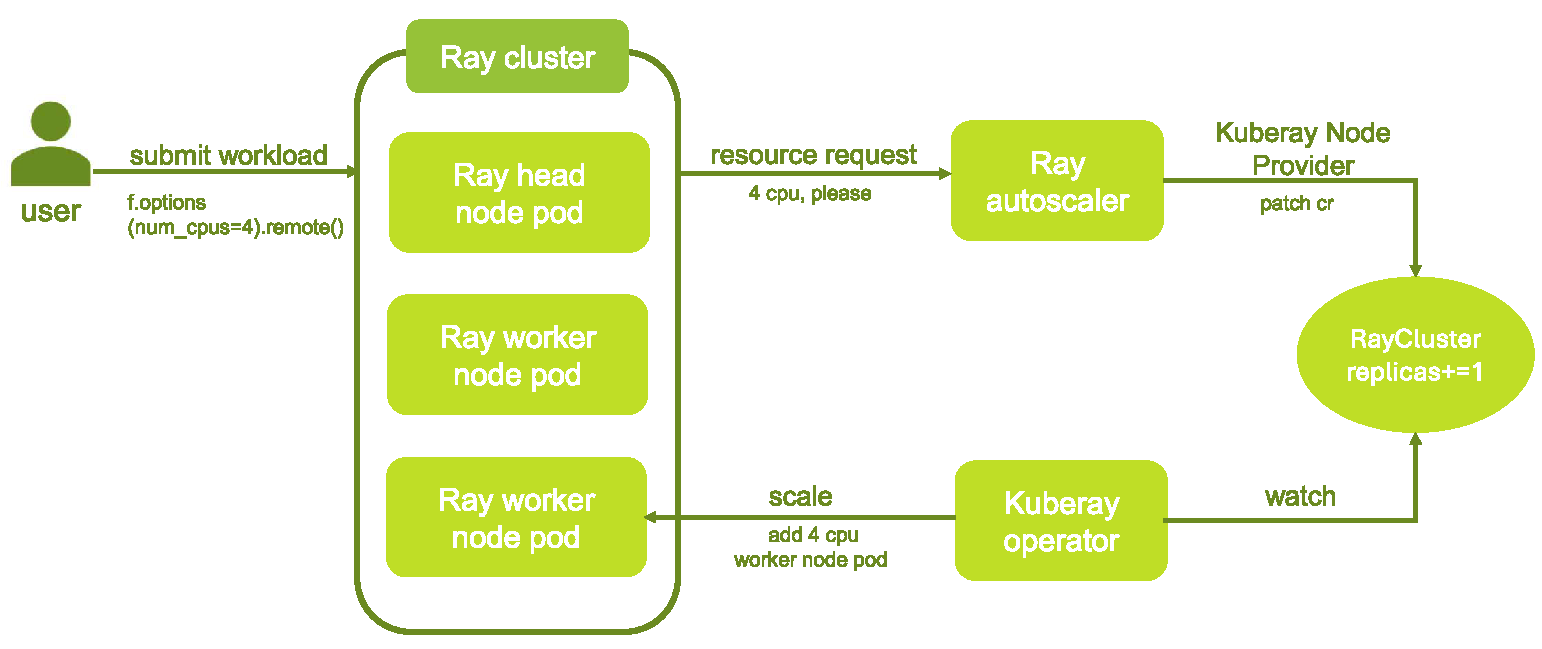
\includegraphics[width=1 \linewidth]{Thesis/Figures/Slide13.pdf}
\caption{\label{fig:Autoscaling with Ray}Autoscaling with Ray \cite{ray_doc}}
\end{figure}
